This Software Requirements Specification (SRS) outlines the software and system requirements for Rahguzar, a route optimization project aimed at improving efficiency in retail and distribution. It details functional requirements for system capabilities and non-functional requirements like performance and scalability. The document also includes system block diagrams, use cases, and external interfaces to clarify the system’s design and interactions.

\section{Functional Requirements}


% This section describes each function/feature provided by our system. These functions are logically grouped into modules based on their purpose/users/mode of operations etc (as per our system). A functional hierarchy may look like:

The functional requirements for this system focus on creating an efficient journey-planning solution tailored for order bookers and sales representatives. This system is designed to optimize routes based on key operational parameters and provide dynamic rerouting, while also supporting targeted store visits and frequency schedules. Additional modules include a user-friendly web platform, pilot testing and validation, and performance monitoring to ensure enhanced efficiency and measurable sales impact.The following are the functional requirements for each module and their respective functions.

\subsection*{Module 1: Route Optimization Algorithm}
\subsubsection*{Function 1: Route Generation}
\begin{itemize}
    \item Implement an algorithm that creates journey plans optimized for order bookers and sales representatives.
    \item The optimization should consider multiple factors:
    \begin{itemize}
        \item[] \textbf{Sub Function 1: Order Booker Shift Times} \\
            Align route planning with the working hours of each order booker.
        \item[] \textbf{Sub Function 2: Number of Shops to Visit} \\
            Adjust routes to maximize the number of shops visited within constraints.
        \item[] \textbf{Sub Function 3: Number of Order Bookers Available} \\
            Allocate routes based on the number of available staff.
        \item[] \textbf{Sub Function 4: Total Distance Traveled} \\
            Minimize the total distance covered during journeys.
        \item[] \textbf{Sub Function 5: Total Travel Time} \\
            Reduce the time taken to complete the planned routes.
        \item[] \textbf{Sub Function 6: Store Service Times} \\
            Account for different service time requirements at each store.
    \end{itemize}
\end{itemize}

\subsubsection*{Function 2: Dynamic Rerouting}

    % \item Integrate a feature to adjust routes based on updated data (e.g., traffic, store closure).
    % \item The rerouting should optimize new paths instantly to maintain efficiency.

    \begin{itemize}
        \item It allows users to adjust the generated routes based on their preferences. They can move stores between order bookers and modify store status (e.g., active/inactive).
        \item It simply enables real-time rerouting, with the algorithm instantly updating the allocation of stores and route paths to reflect user preferences, providing flexibility and adaptability in journey planning.
    \end{itemize}

 

% \subsection*{Module 2: Weekly Store Visit Optimization 
% }

\subsubsection*{Function 3: Store Visit Frequency: 
}

\begin{itemize}
    \item Design the algorithm to include visit frequency for each store (e.g., once, twice a week).
    \item Ensure that the routes align with required visit frequencies without any overlap and maintains at least a 3 day gaps between repeated visits.
\end{itemize}

\subsubsection*{Function 4: Journey Planning for Different Timeframes: 
}

\begin{itemize}
    \item Support the generation of routes 
by allowing custom day plan creation and enable downloads for extended periods, based on the target timeframe.
    \item Ensure that stores are scheduled accurately according to their frequency needs while minimizing travel and maximizing coverage.
\end{itemize}



 

% \subsection*{Module 3: Store Profile Management and Integration }

\subsubsection*{Function 5: Store Profiling: }

\begin{itemize}
    \item Maintain detailed profiles for each store, including:
    \begin{itemize}
        \item[] \textbf{Sub Function 1:} Geographical hierarchy (region, zone, territory, town).
        \item[] \textbf{Sub Function 2:} Sales channel type (e.g., wholesale or retail).
    \end{itemize}
    \item Enable users to filter stores by parameters like region, sales channel, or visit frequency. Allow custom filters linked to all stores by uploading relevant data (e.g., location, sales volume), enabling dynamic application across stores. This approach enhances flexibility and control in route optimization.
    \item Enable users to modify store status (active/inactive) directly within the system.
\end{itemize}

\subsubsection*{Function 6: Targeted Journey Plans:}
 
\begin{itemize}
    \item Enable the system to generate routes targeting specific store types (e.g., only wholesale stores in a particular region).
    \item Allow users to select areas and stores for targeted visits, ensuring that the algorithm generates routes based on these selections.
\end{itemize}

 

\subsection*{Module 2: Web Application Platform 
}

\subsubsection*{Function 1: User Interface for Route Management: 
}

\begin{itemize}
    \item Create a user-friendly web interface for managers to access and manage journey plans.
\end{itemize}
\subsubsection*{Function 2: Integrate Map Interface:
}

    \begin{itemize}
        \item Designing, viewing, and adjusting routes.
        \item Displaying essential shop details (e.g., store profiles, geographical location).
        \item Defining and viewing boundaries like regions, territories, and areas.
    \end{itemize}

\subsubsection*{Function 3: Manual Override and Adjustment: 
}

\begin{itemize}
    \item Provide a manual override feature that allows managers to adjust routes manually.
    \item Include input options for master data (store profiles, visit frequencies, geographical details) directly within the platform.
\end{itemize}

\subsubsection*{Function 4: Downloadable Reports: 
}

\begin{itemize}
    \item Allow users to export optimized or manually adjusted routes in a downloadable format for offline analysis or distribution.
\end{itemize}

\subsection*{Module 3: Pilot Testing and Validation }

\subsubsection*{Function 1: Test Plan Creation: 
}

\begin{itemize}
    \item Develop a comprehensive pilot testing framework to validate the system's effectiveness.
\end{itemize}
\subsubsection*{Function 2: Real-World Data Integration: }

\begin{itemize}
    \item Gather real-world data during pilot testing, ensuring data is accurate and reliable.
\end{itemize}

\subsubsection*{Function 3: Performance Assessment: }
\begin{itemize}
    \item Collect and analyze data (travel time, number of shops visited, sales impact, etc.) to assess system performance.
    \item Implement an adjustment process based on pilot feedback to enhance the algorithm.
\end{itemize}

\subsubsection*{Function 4: Case Study Development: }

\begin{itemize}
    \item Compile a case study summarizing the outcomes, findings, and system performance.
\end{itemize}

\subsection*{Module 4: Performance Monitoring and Reporting }

\subsubsection*{Function 1: Key Performance Indicators (KPIs): }

\begin{itemize}
    \item Track and display metrics like:
\end{itemize}
    \begin{itemize}
    \item[] \textbf{Sub Function 1:} Average travel time per route.
    \item[] \textbf{Sub Function 2:} Number of shops visited per shift.
    \item[] \textbf{Sub Function 3:} Number of order bookers required per distribution.
    \item[] \textbf{Sub Function 4:} Sales uplift due to route optimization.
    \item[] \textbf{Sub Function 5:} Algorithm response time for route recalculations.
\end{itemize}
 

\subsubsection*{Function 3: Metrics Dashboard:
}

\begin{itemize}
    \item Develop a dashboard to visualize KPIs, providing insights into efficiency improvements, time savings, and sales increases.
\end{itemize}




% --- The above is to be modified as per your project, e.g. a flat list if your system has limited functional requirements.

\section{Non-functional Requirements}

% This sections mentions the specific non-functional requirements of our system. These generally address performance, scalability, safety, availability, deployment etc.

The Non-functional requirements define the quality and performance attributes of this system, focusing on scalability, usability, and reliability. They ensure optimal performance under varying conditions while maintaining data security and adaptability for user needs. Additionally, following requirements also facilitate maintainability for future enhancements, ensuring the system remains effective over time.



\begin{enumerate}
    \item \textbf{Scalability, Efficiency, and Memory Optimization}
    \begin{itemize}
        \item The system is designed to efficiently handle large datasets and scale up to 1000+ stores effectively as the amount of data increases, ensuring optimal performance and quick response times within 2 minutes for route generation.
        \item It should also have a low memory footprint, ensuring that it can scale effectively without degrading system performance or requiring excessive computational resources.
    \end{itemize}
    
    \item \textbf{Usability}
    \begin{itemize}
        \item A user-friendly web application interface is required, allowing users to manage, optimize, and adjust journey plans easily.
        \item The map interface must provide intuitive visualization and interactivity for planning and real-time adjustments.
    \end{itemize}
    
    \item \textbf{Reliability and Performance}
    \begin{itemize}
        \item The optimization algorithm should be robust, quickly generating optimal routes based on parameter changes, such as order booker shifts or the number of stores per booker.
        \item The system should maintain a minimum uptime of 95\%, allowing for up to 36 hours of downtime per month for a smooth user experience.
        
    \end{itemize}
    
    \item \textbf{Security}
    \begin{itemize}
        \item Data security protocols should protect sensitive information such as store profiles and geographical hierarchies, especially when integrating third-party APIs.
        \item User authentication mechanisms should be implemented to ensure that only authorized personnel can access sensitive data and functionalities within the system.

    \end{itemize}
    
    \item \textbf{Adaptability and Flexibility}
    \begin{itemize}
        \item Manual override functionality should allow users to adjust routes when needed, ensuring flexibility in route planning.
        \item The system should support long-term planning options, including daily, weekly, or monthly route generation and optimization.
    \end{itemize}
    
    \item \textbf{Maintainability}
    \begin{itemize}
        \item The architecture should allow for future enhancements, such as integrating additional parameters or algorithms for optimization, without significant rework.
    \end{itemize}
    
\end{enumerate}

\section{External Interfaces}

% We expect every project to have at least of the following subsections. This section must be aligned with your project deliverables. Please consult with your project supervisor regarding which of the following section(s) you should include in your report

\subsection{User Interfaces}
The Web application interface is designed to be user-friendly and intuitive, allowing managers to easily navigate through the system. The interface includes various features such as route management, store profiling, and performance monitoring. The design focuses on providing a seamless experience for users, enabling them to efficiently manage their journey plans and access relevant data.

\begin{figure}[H]
    \centering
    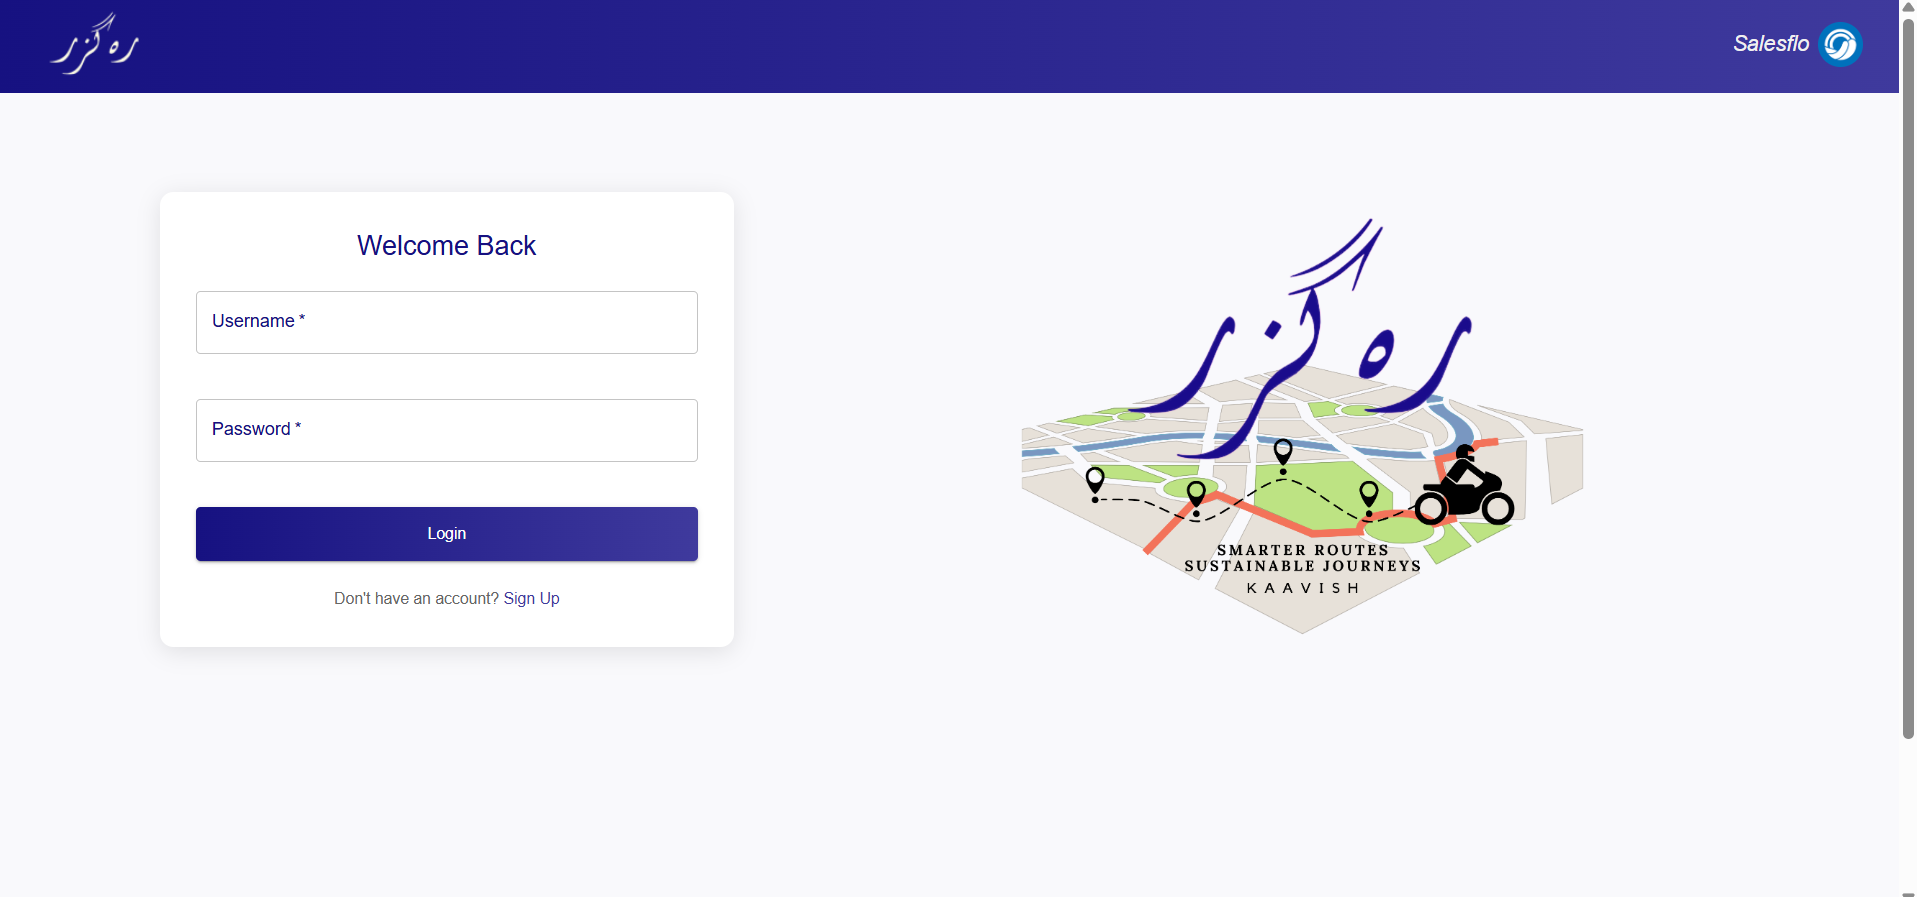
\includegraphics[width=1\textwidth]{images/Login.png} % Adjust width as needed
    \caption{Login Screen}
    \label{fig:image1}
\end{figure}
The login screen is shown in Figure~\ref{fig:image1}, letting the user enter their username and password to login.


\begin{figure}[H]
    \centering
    \includegraphics[width=1\textwidth]{images/StartScreen.png} % Adjust width as needed
    \caption{Home Page}
    \label{fig:image3}
\end{figure}
The ``Home Page" screen is shown in Figure~\ref{fig:image3}. The Route plan generator is the main screen where the instructions to start are provided.


\begin{figure}[H]
    \centering
    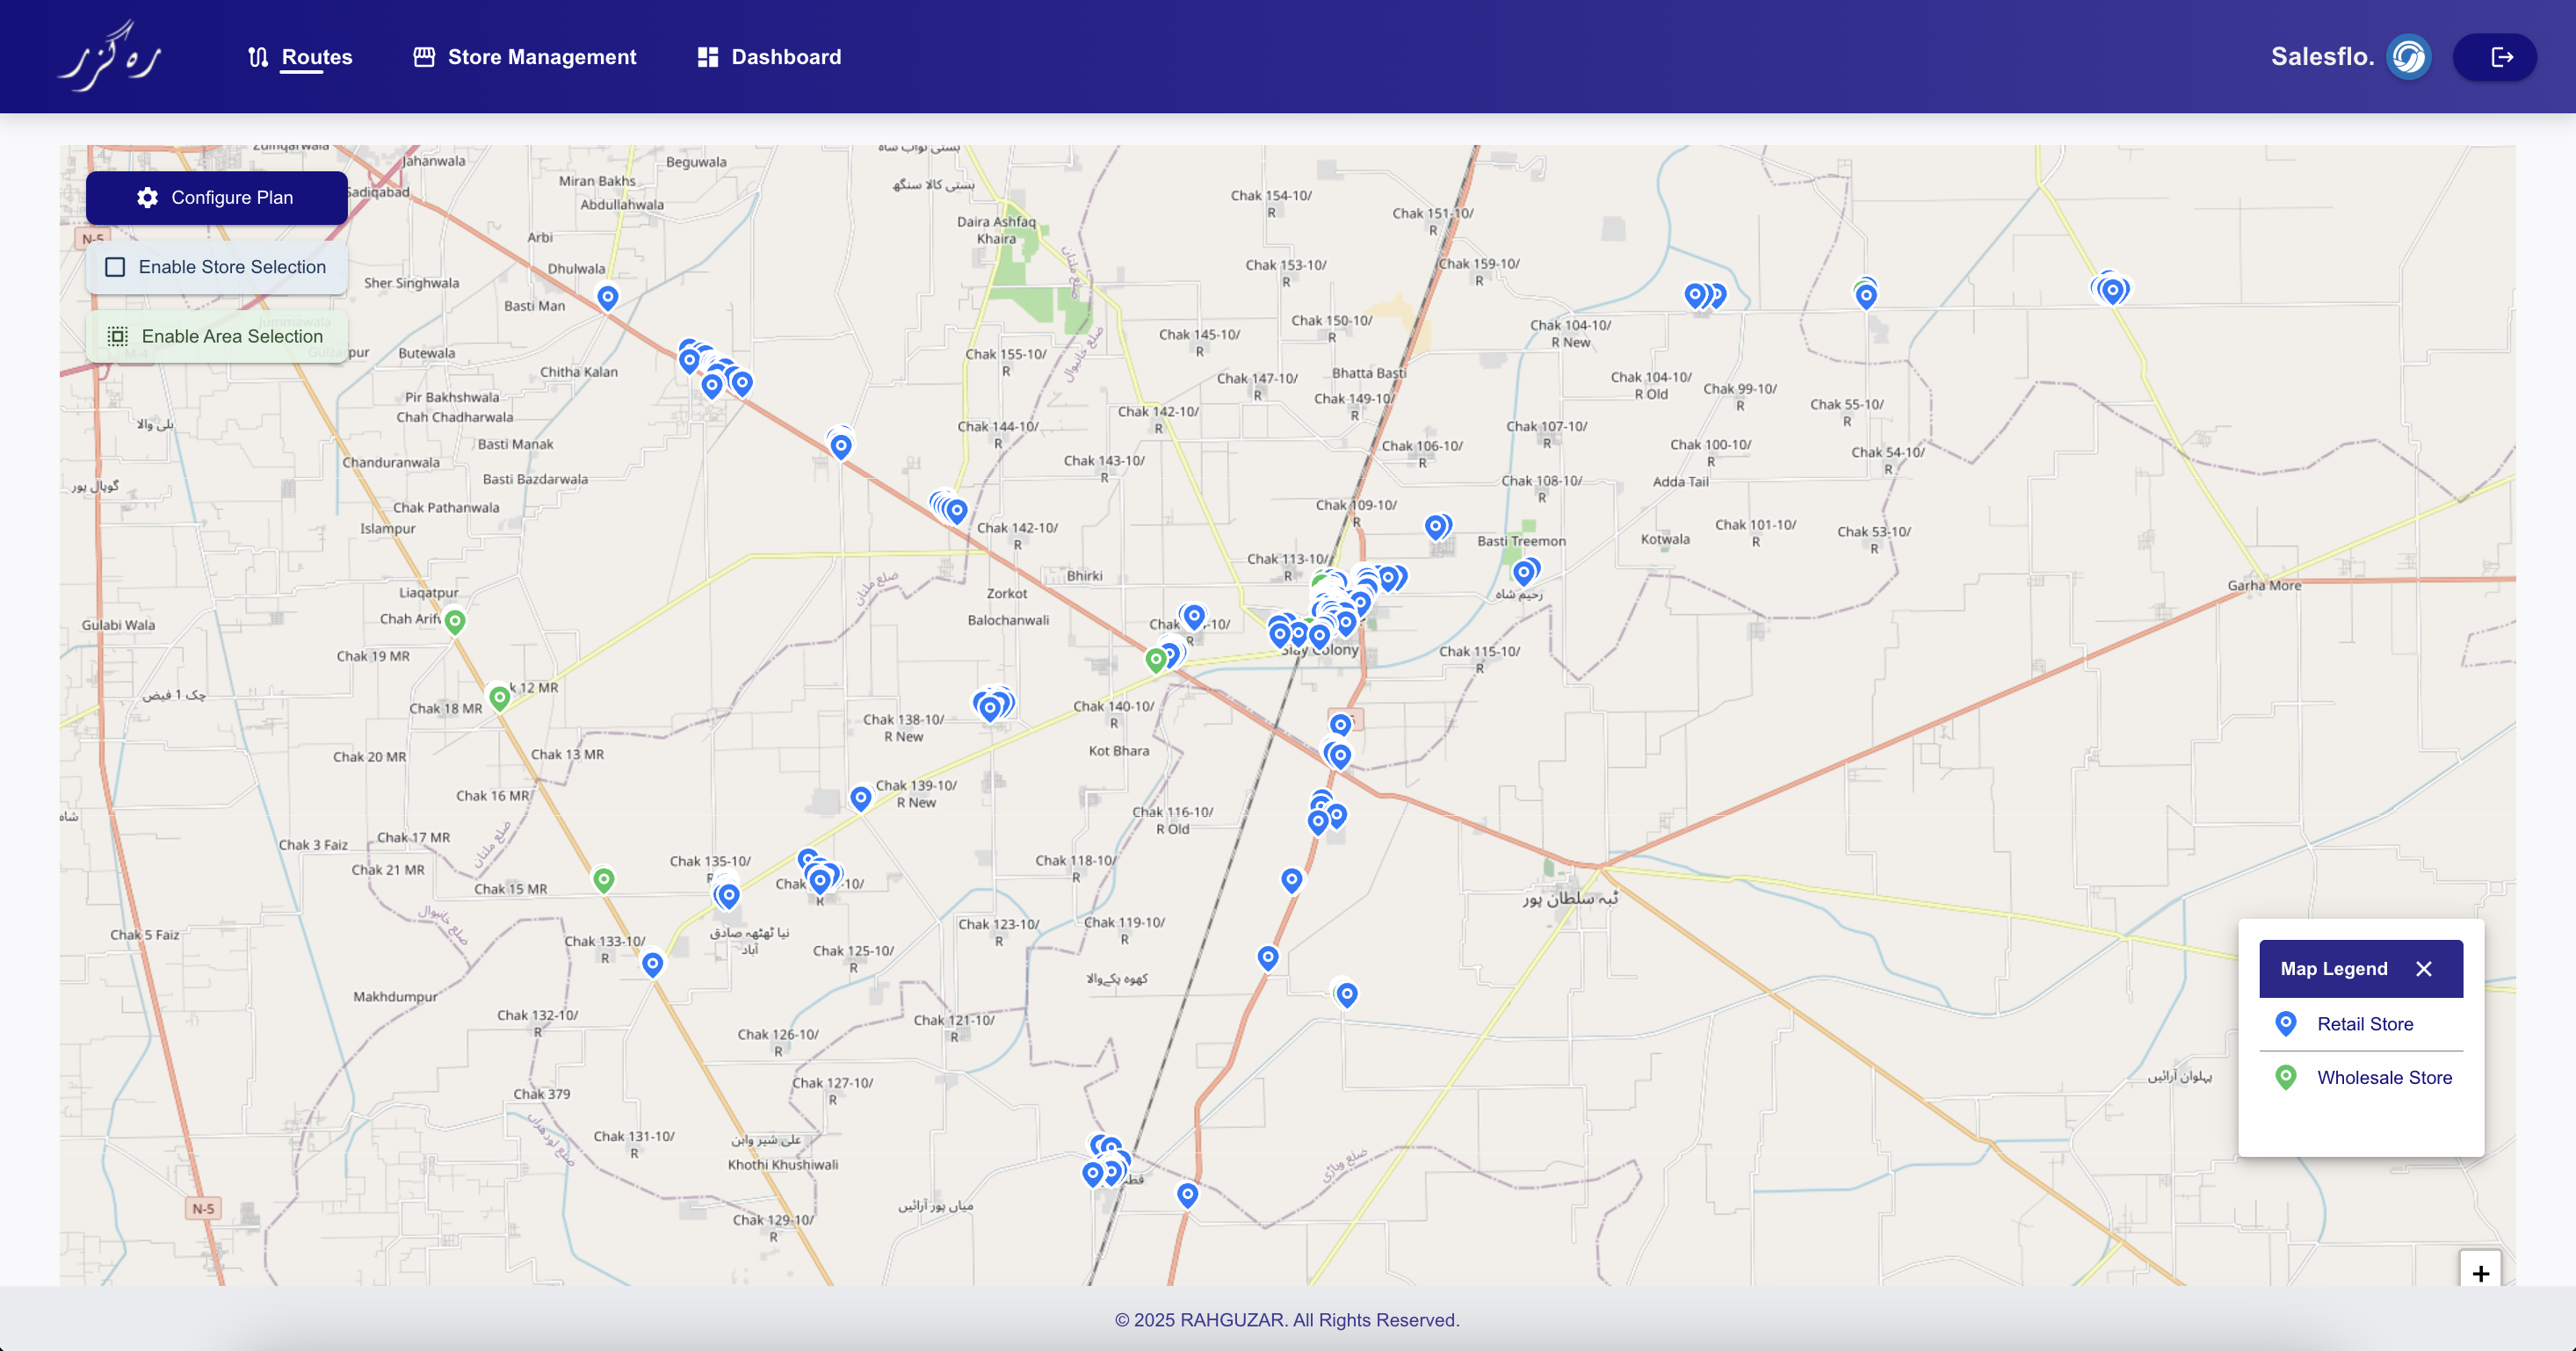
\includegraphics[width=1\textwidth]{images/Map.png} % Adjust width as needed
    \caption{Plan Route Page}
    \label{fig:image4}
\end{figure}
The ``Map" screen is shown in Figure~\ref{fig:image4}. In this screen, the manager will be able to view the map and the stores on it. The manager can select stores using area selection or point selection which will be used in the plan.


\begin{figure}[H]
    \centering
    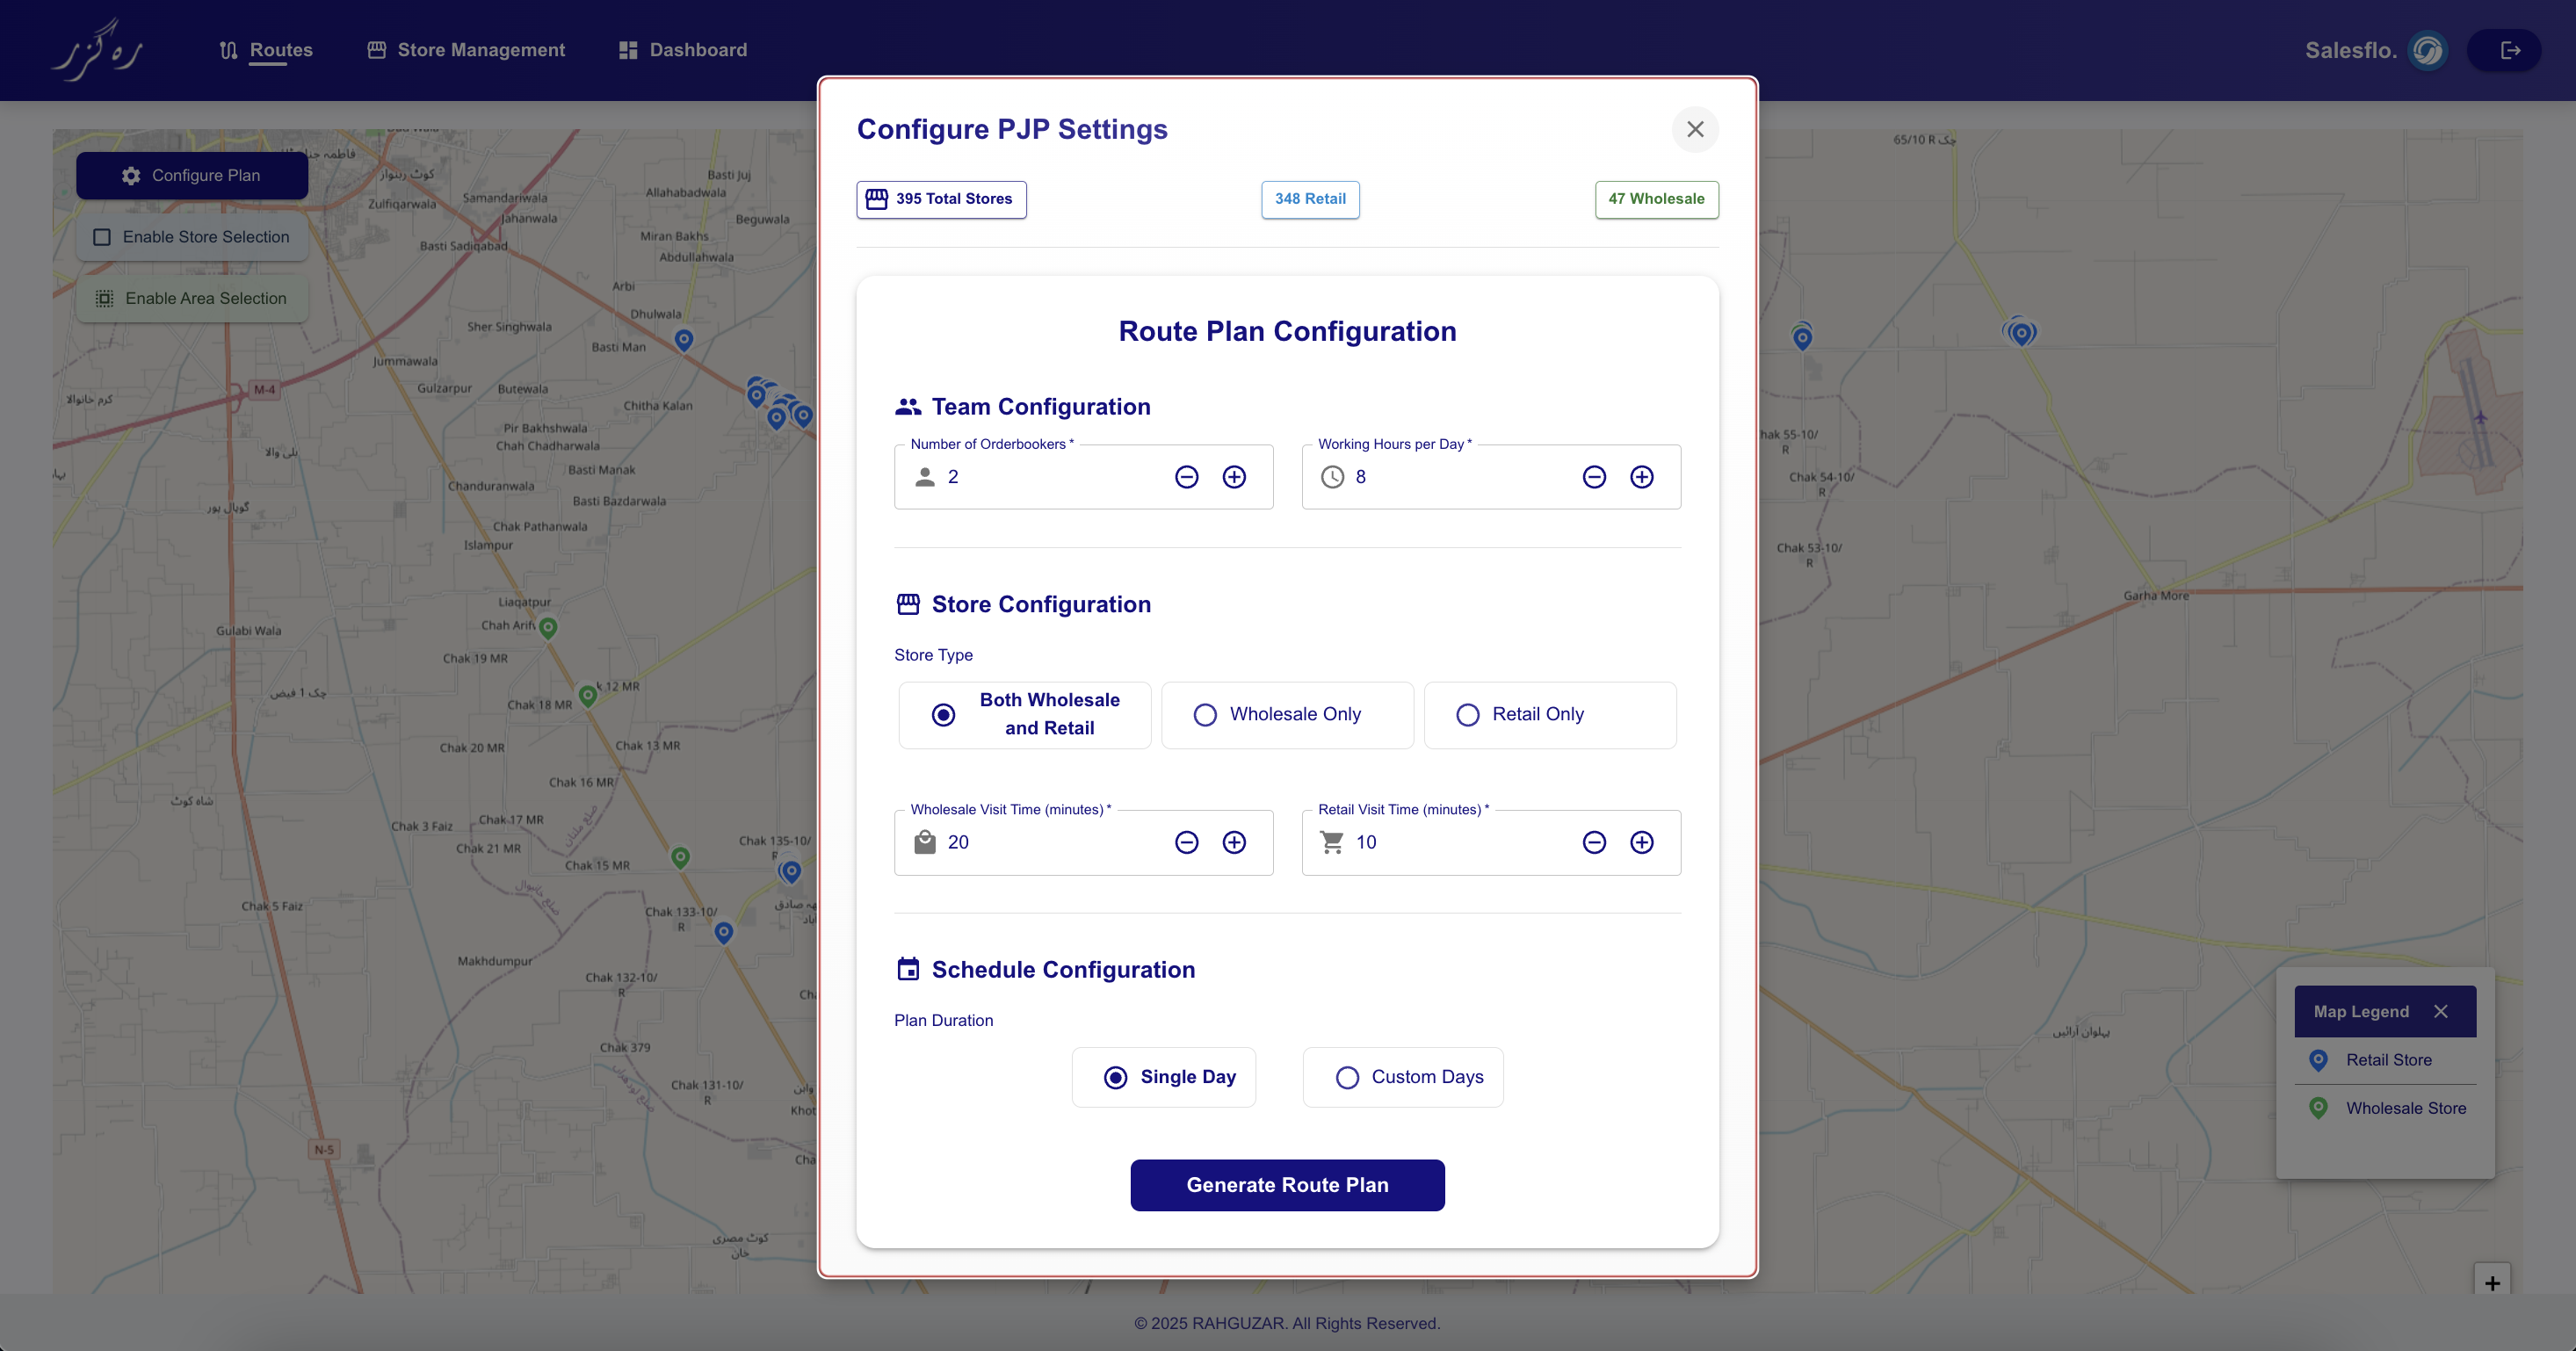
\includegraphics[width=1\textwidth]{images/Configure.png} % Adjust width as needed
    \caption{Configure Route Parameters}
    \label{fig:image4}
\end{figure}
The manager can configure the route parameters in the ``Configure Route" screen shown in Figure~\ref{fig:image4}. In this screen, the manager will be able to set the shift timings, number of order bookers, and the number of stores to visit. The manager can also set the travel time and service time for each store.

\begin{figure}[H]
    \centering
    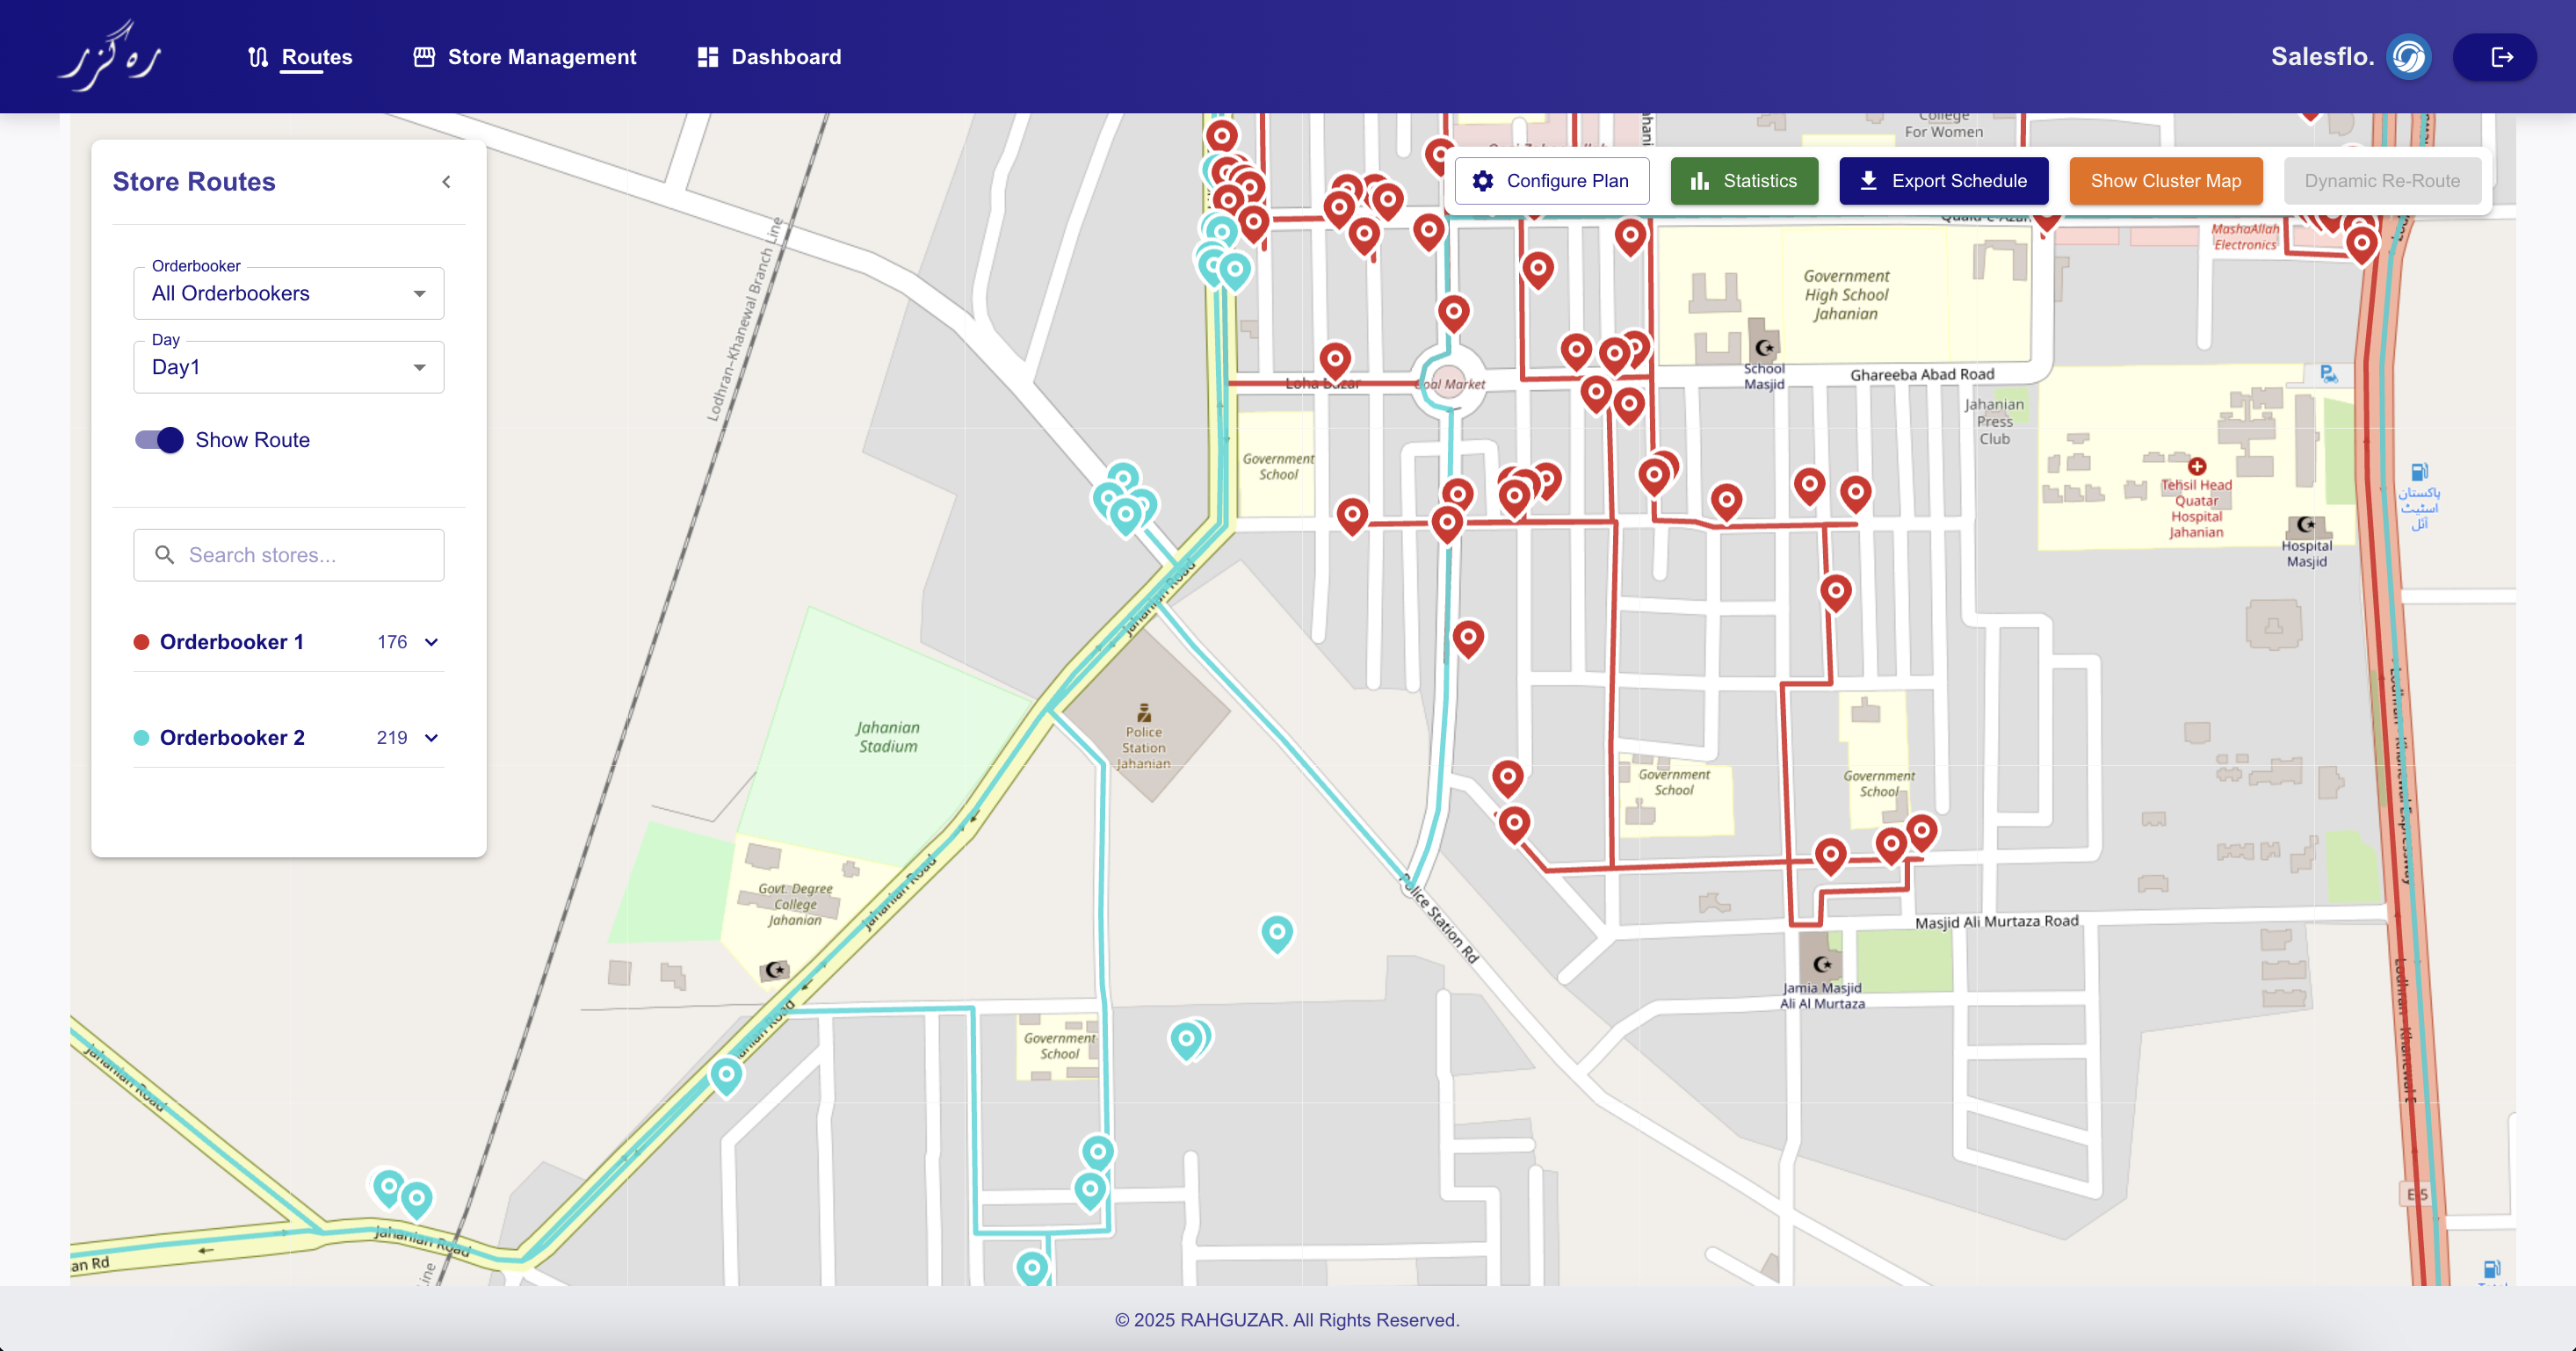
\includegraphics[width=1\textwidth]{images/plan.png} % Adjust width as needed
    \caption{View Routes Page}
    \label{fig:image6}
\end{figure}
The ``Plan Route" screen is shown in Figure~\ref{fig:image6}. In this screen, the manager will be able to view the routes generated by the system. The manager can also view the route details such as the distance, travel time, and service time for each store. The manager can also view the route on the map and download it in a CSV format.

\begin{figure}[H]
    \centering
    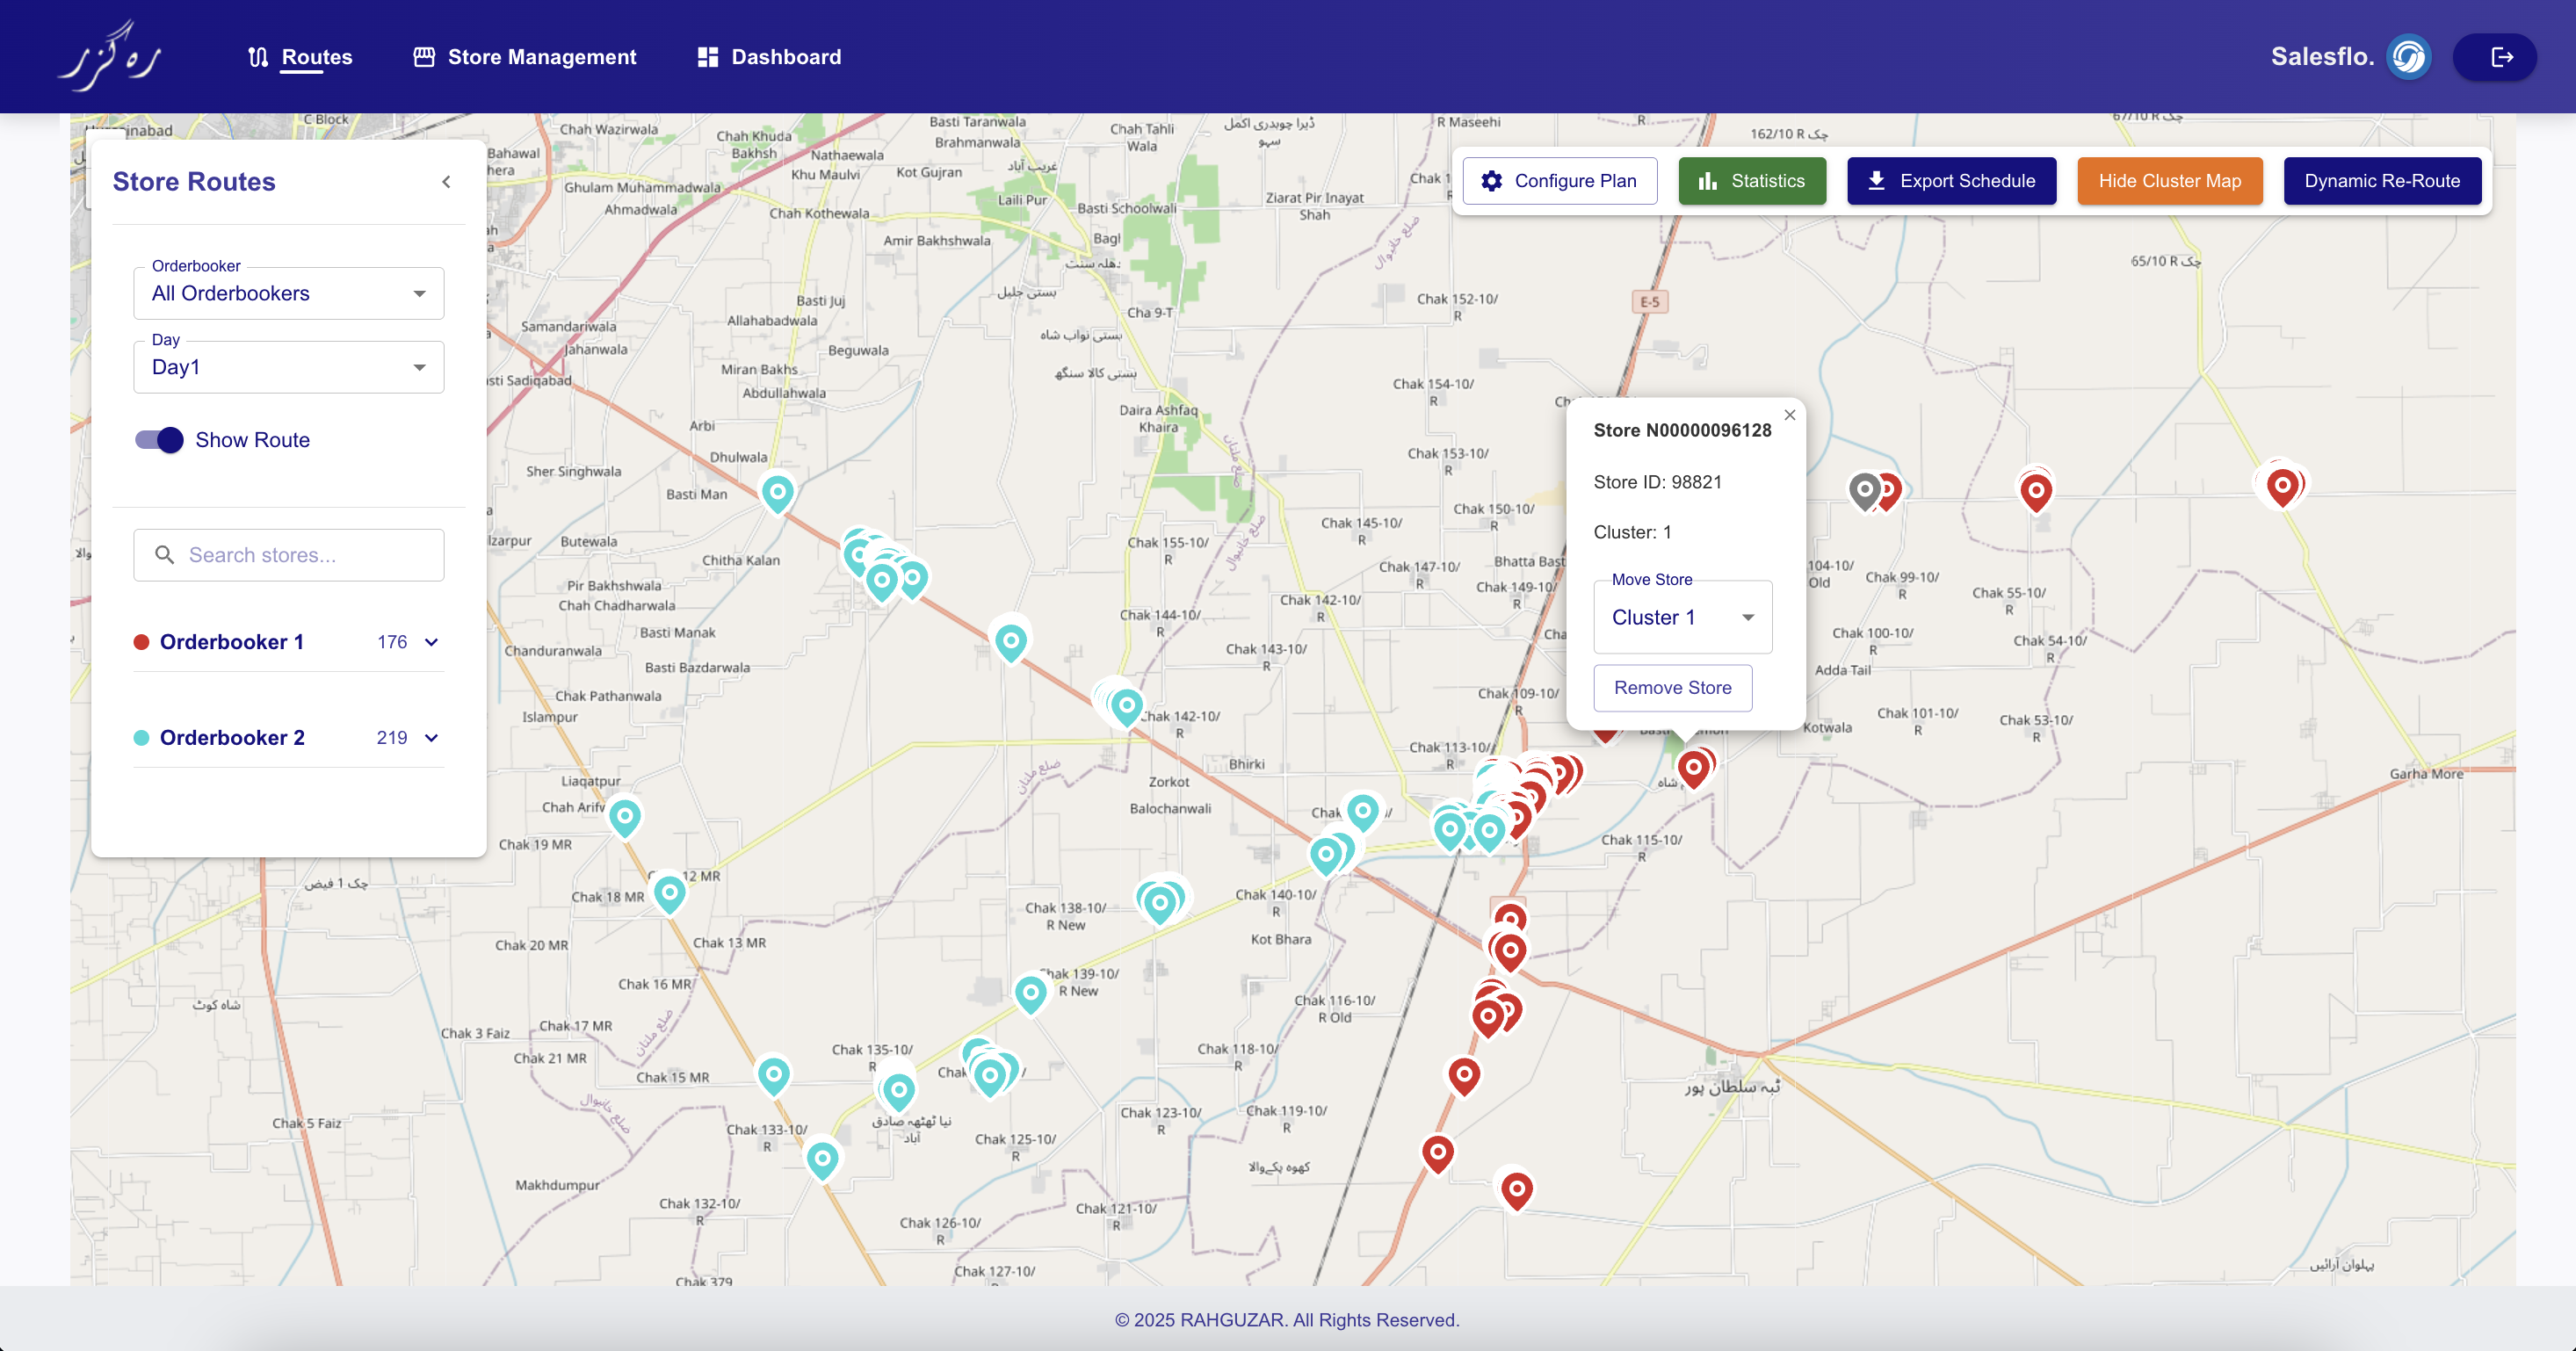
\includegraphics[width=1\textwidth]{images/Clustermap.png} % Adjust width as needed
    \caption{Cluster Map Page}
    \label{fig:image6}
\end{figure}
The ``Cluster Map" screen is shown in Figure~\ref{fig:image6}. In this screen, the manager will be able to view the clusters generated by the system. The manager can modify the stores in clusters by removing them or moving them to another cluster, after which they can dynamically reroute the plan.

\begin{figure}[H]
    \centering
    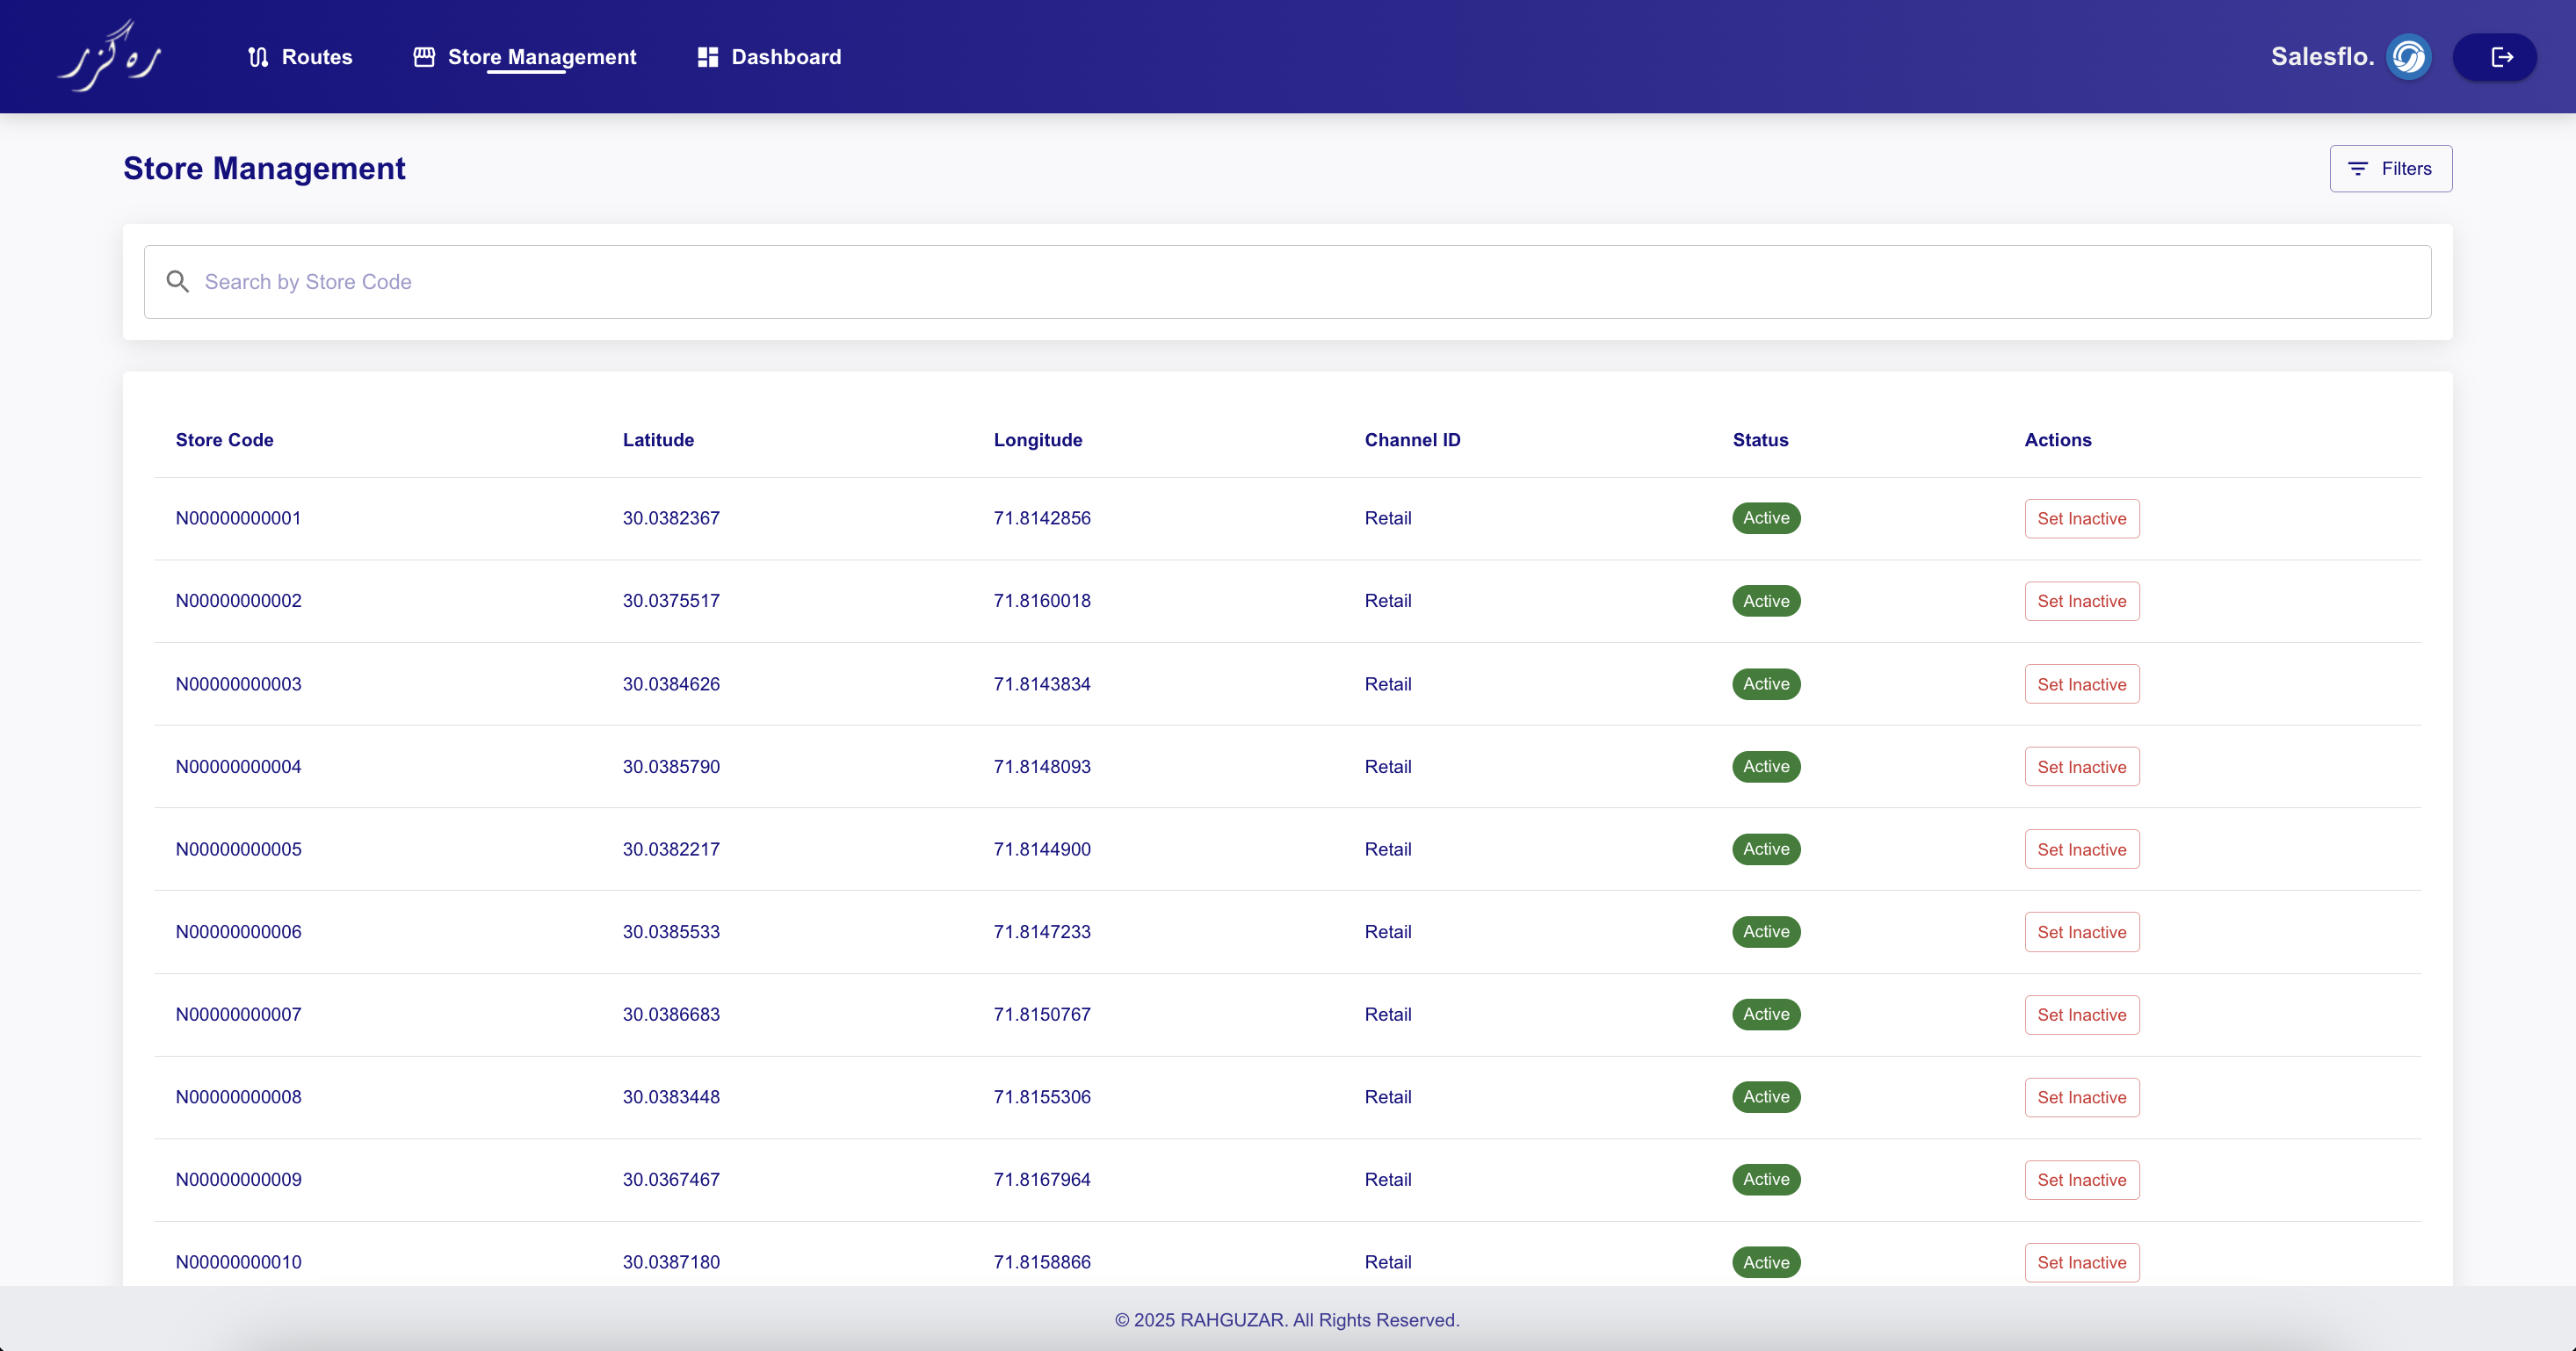
\includegraphics[width=1\textwidth]{images/stores.png} % Adjust width as needed
    \caption{Stores Management Page}
    \label{fig:image5}
\end{figure}
The "Stores Management" screen is shown in Figure~\ref{fig:image5}. In this screen, the manager will be able to search a certain store, apply filters in their search, and view its information such as its coordinates. The manager has the option to view more than 1 store's information at a time, and to decide to set a store active or inactive.

\begin{figure}[H]
    \centering
    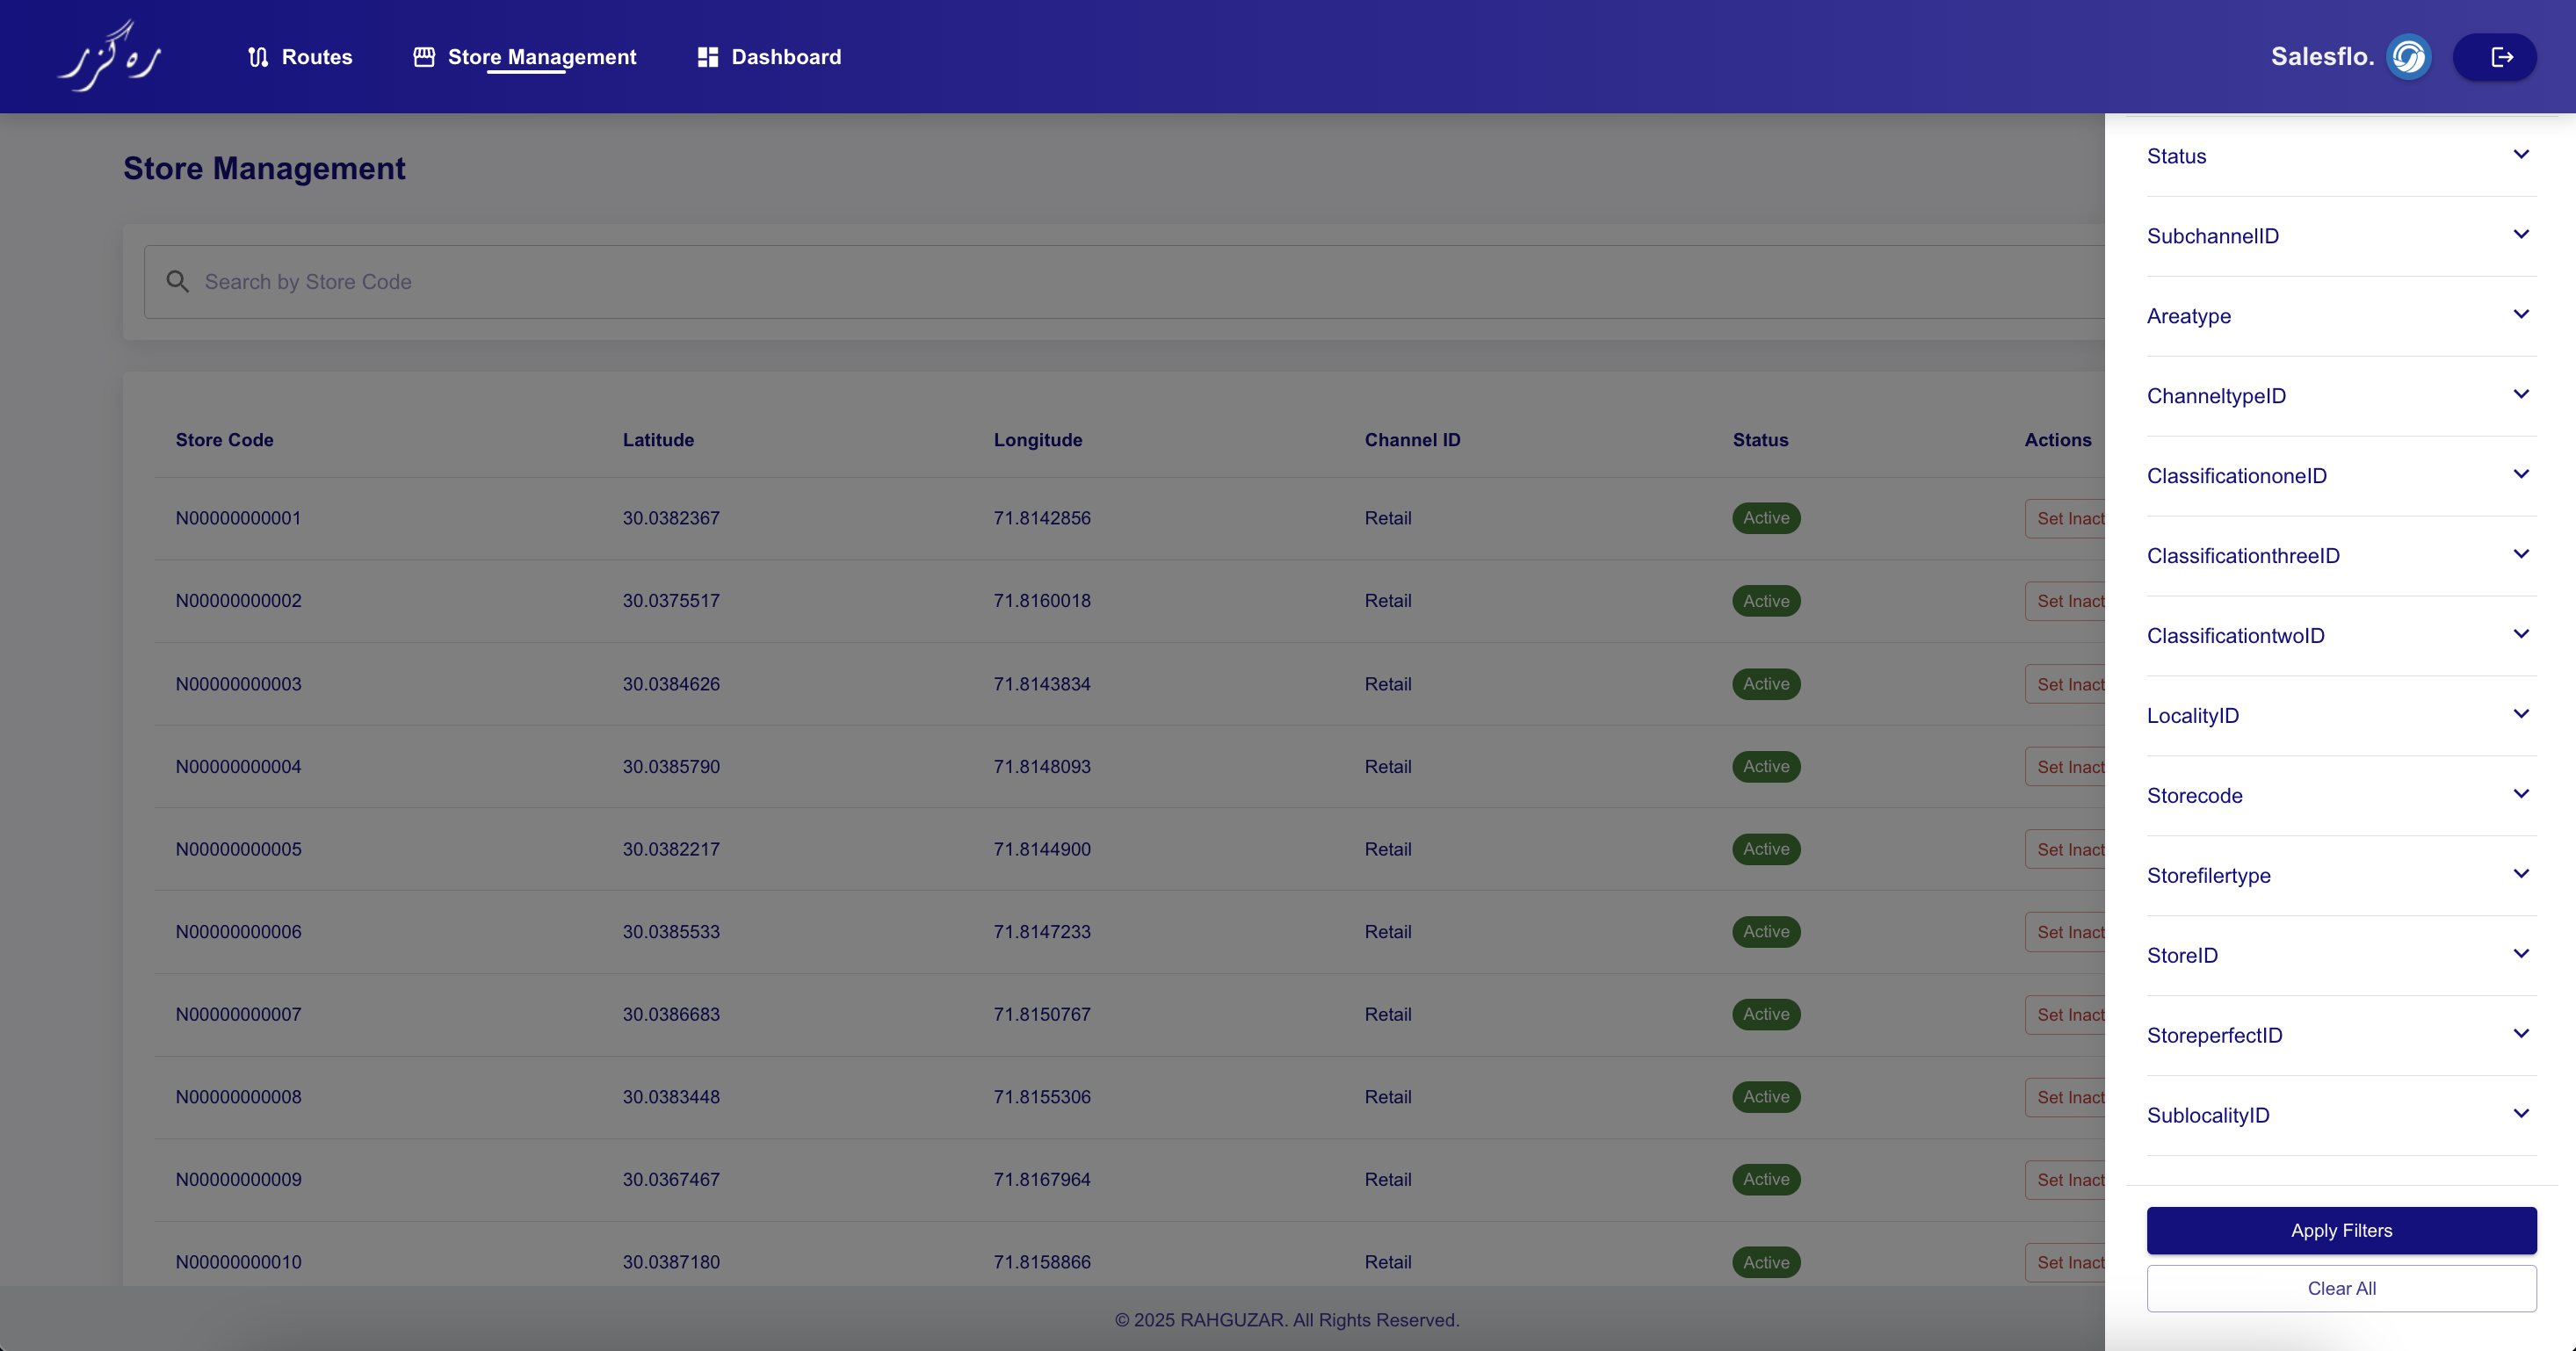
\includegraphics[width=1\textwidth]{images/store filters.png} % Adjust width as needed
    \caption{Store Filters}
    \label{fig:image6}
\end{figure}
The ``Store Filters" screen is shown in Figure~\ref{fig:image6}. In this screen, the manager will be able to view the filters applied to the stores.

\begin{figure}[H]
    \centering
    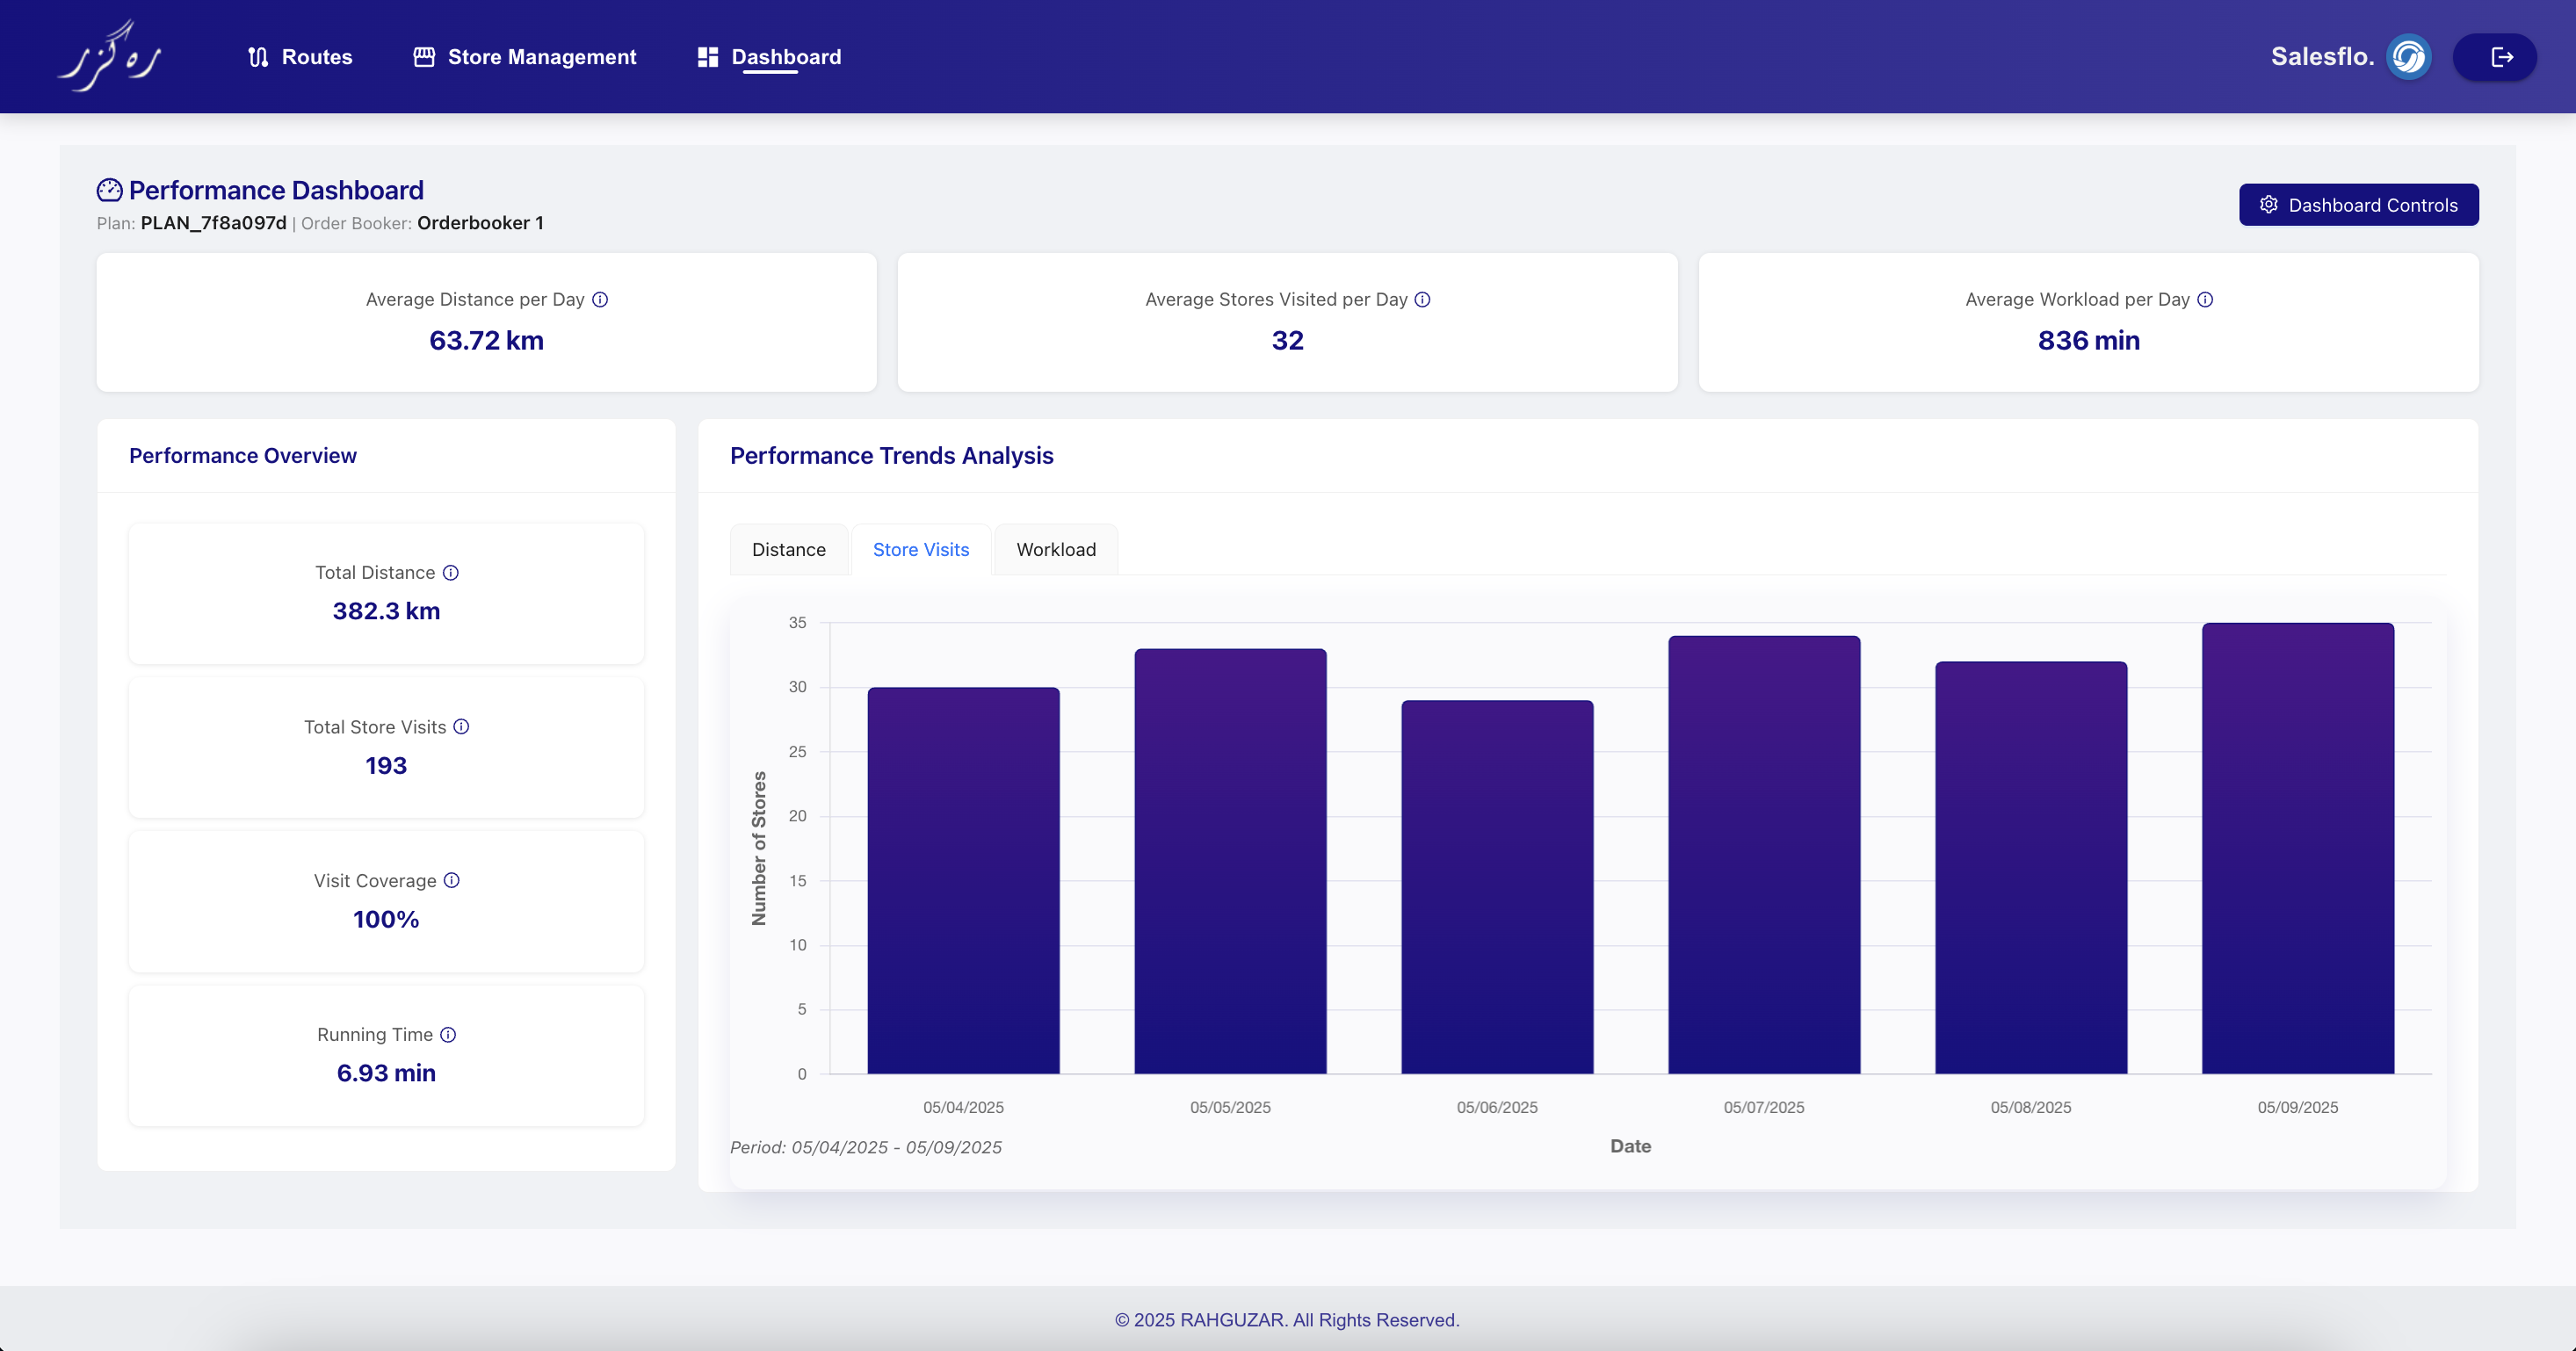
\includegraphics[width=1\textwidth]{images/dashboard.png} % Adjust width as needed
    \caption{Dashboard Page}
    \label{fig:image7}
\end{figure}
The ``Dashboard" screen is shown in Figure~\ref{fig:image7}. In this screen, the manager will be able to view certain KPIs that indicate the overall performance of the routes such as Average Daily Distance and Workload per Representative, Average travel time per per orderbooker or over all orderbookers. 

\subsection{Application Program Interface (API)}
The API layer is the backbone of the Rahguzar system, enabling seamless communication between the frontend, backend, and external services. Designed using REST principles, the API ensures efficient data exchange, operational scalability, and secure access control.

\subsubsection{REST API Endpoints}
The system is built with RESTful API endpoints that manage data transfer between components. Key endpoints include:

\begin{itemize}
    \item \textbf{Route Management Endpoints:}
    \begin{itemize}
        \item \texttt{POST /optimize} — Submits parameters to generate optimized journey plans.
        \item \texttt{POST /reroute-clusters} — Dynamically reassigns stores and reroutes OBs.
        \item \texttt{GET /get\_routes} — Retrieves finalized optimized routes.
    \end{itemize}

    \item \textbf{Store Profile Endpoints:}
    \begin{itemize}
        \item \texttt{GET /api/stores} — Fetches all store profiles.
        \item \texttt{POST /assign\_store} — Assigns a store to an order booker.
        \item \texttt{PUT /api/stores/\{store\_id\}} — Updates metadata of a specific store.
    \end{itemize}

    \item \textbf{Dashboard and KPI Endpoints:}
    \begin{itemize}
        \item \texttt{GET /get\_kpi\_data} — Returns key performance indicators.
        \item \texttt{GET /get\_graph\_data} — Fetches time-series analytics for visualization.
    \end{itemize}
\end{itemize}

\subsubsection{Authentication and Authorization}
To secure API access, the Rahguzar system employs JWT (JSON Web Tokens) for user authentication.

\begin{itemize}
    \item \texttt{POST /login} — Authenticates user credentials and returns a JWT token.
    \item \textbf{Token Usage:} The JWT token must be attached to the \texttt{Authorization} header as \texttt{Bearer <token>} in all subsequent API requests.
\end{itemize}

\subsubsection{External Services Integration}
To support essential routing and mapping functionalities, the system integrates with third-party services:

\begin{itemize}
    \item \textbf{Open Source Routing Machine (OSRM):}
    \begin{itemize}
        \item Dockerized and hosted on an EC2 instance for internal routing.
        \item \textbf{Endpoint:} \texttt{GET /route/v1/driving/\{lon,lat;lon,lat,...\}} — Returns route geometry and travel metadata in GeoJSON format.
    \end{itemize}
\end{itemize}

\subsubsection{Route Optimization Engine}
The route optimization component is embedded in the backend, using hybrid algorithms for clustering, scheduling, and routing.

\begin{itemize}
    \item \textbf{Python + OR-Tools:} Implements clustering, scheduling and route generation logic using Evolutionary Algorithms and TSP solvers.
\end{itemize}

\subsubsection{Data Storage and Synchronization}
The system utilizes a relational data model hosted on AWS RDS using PostgreSQL.

\begin{itemize}
    \item \textbf{PostgreSQL (via RDS):} Stores all persistent data including users, stores, routes, plans, and KPI metrics.
    \item \textbf{Synchronization Mechanisms:} Data flows between backend modules and frontend views are synchronized via well-defined API transactions and database-level consistency checks.
\end{itemize}

\subsubsection{Data Monitoring}
To enable effective monitoring, the API supports data updates and performance tracking:

\begin{itemize}
    \item \textbf{Performance Analytics:} Endpoints such as \texttt{/get\_kpi\_data} and \texttt{/get\_graph\_data} provide real-time insights on route efficiency, travel time, visit compliance, workload distribution, and other KPIs to support ongoing performance tuning and planning.
\end{itemize}



\subsection{Hardware/Communication Interfaces}
Our System relies on specific hardware and communication protocols to ensure seamless operation and efficient data management.

\subsubsection{Client-Side Hardware Requirements}
Manager Workstations: Managers access the system through web browsers on desktops or laptops for route planning and monitoring. Recommended specifications include:
\begin{itemize}
    \item \textbf{Processor:} Dual-core or higher.
    \item \textbf{RAM:} 4GB minimum.
    \item \textbf{Internet Connection:} Stable broadband with at least 5 Mbps for real-time data processing.
    \item \textbf{Browser Compatibility:} Supports modern web browsers like Chrome, Firefox, and Edge.
\end{itemize}

\subsubsection{Server-Side Infrastructure}
The backend and database components are hosted on cloud infrastructure (AWS) to ensure availability, fault tolerance, and scalability.

\begin{itemize}
    \item \textbf{Application Server (EC2):}
    \begin{itemize}
        \item Hosted on an Amazon EC2 instance (e.g., t3.medium or higher).
        \item Runs the Flask-based backend application, route optimization engine, and API endpoints.
        \item Configured with Gunicorn and optionally Nginx for request handling and reverse proxy.
        \item Operating System: Ubuntu Server 20.04 LTS or equivalent.
    \end{itemize}

    \item \textbf{Database Server (RDS):}
    \begin{itemize}
        \item PostgreSQL instance managed via Amazon RDS.
        \item Stores all system data including user credentials, store metadata, plan configurations, route outputs, and KPI records.
        \item SSD-based storage with automated backup and optional multi-AZ redundancy.
    \end{itemize}

    \item \textbf{Storage:} EC2 instance uses SSD storage for intermediate computation results and application logs.

    \item \textbf{Networking:} Secured via AWS security groups. Backend accessible via HTTPS; database accessible only through private IPs or controlled access rules.
\end{itemize}

\subsubsection{Communication Interfaces}
\begin{itemize}
    \item \textbf{Internet Connection:} All interactions between the frontend and backend rely on a stable internet connection for data synchronization and API requests.
\newpage
    \item \textbf{Data Communication Protocols:}
    \begin{itemize}
        \item \textbf{HTTPS:} Secure communication between frontend, backend, and external services like Google Maps API.
        \item \textbf{API Calls:} RESTful API requests enable data transfer for route management, visit updates, and user authentication.
    \end{itemize}
\end{itemize}

\subsubsection{Routing Service (Dockerized OSRM)}
The system utilizes a containerized instance of the Open Source Routing Machine (OSRM) to compute real-world travel distances and generate accurate road-based routes.

\begin{itemize}
    \item \textbf{Deployment Method:} OSRM is deployed via Docker on an EC2 instance to ensure isolation, portability, and ease of deployment.
    \item \textbf{Routing Backend:} Based on preprocessed OpenStreetMap data using the `osrm-backend` image.
    \item \textbf{Port Configuration:} Accessible via HTTP on port 5002 internally, secured behind firewall rules.
    \item \textbf{Container Runtime:} Docker Engine on Ubuntu Server.
    \item \textbf{Data Source:} OSM PBF file for the region of operation (e.g., Pakistan or selected city).
    \item \textbf{Use Case Integration:} Accessed by the backend during route optimization to compute driving distances between stores.
\end{itemize}



\section{Use Cases}
\begin{itemize}
    \item \textbf{User Authentication and Access Control}
    \begin{itemize}
        \item \textbf{Description:} Ensure secure access to the system for both managers and field staff.
        \item \textbf{Actions:}
        \begin{itemize}
            \item As a manager, I want to log in securely to access my dashboard and create journey plans.
            \item As the system, I need to authenticate users to ensure only authorized managers and field staff access the application.
        \end{itemize}
    \end{itemize}
    
    \item \textbf{Route Plan Creation, Configuration, and Optimization}
    \begin{itemize}
        \item \textbf{Description:} Enable the creation of optimized routes based on configurable parameters.
        \item \textbf{Actions:}
        \begin{itemize}
            \item As a manager, I want to create a new optimized route for my field team, configuring parameters like shift timings and visit frequency to align with operational requirements.
            \item As the system, I need to generate optimized routes using parameters such as shift times, visit frequencies, and priorities, ensuring efficient route suggestions for managers.
        \end{itemize}
    \end{itemize}

    \item \textbf{Plan Generation}
    \begin{itemize}
        \item \textbf{Description:} Generate long-term journey plans based on store visit requirements.
        \item \textbf{Actions:}
        \begin{itemize}
            \item As a manager, I want the ability to generate custom day journey plans, providing my team with a consistent schedule for store visits.
            \item As the system, I need to automatically generate journey plans for custom day schedules based on specified visit frequencies.
        \end{itemize}
    \end{itemize}
    
    \item \textbf{Dynamic Rerouting and Manual Overrides}
    \begin{itemize}
        \item \textbf{Description:} Allow for real-time adjustments to routes, either dynamically by the system or manually by the manager.
        \item \textbf{Actions:}
        \begin{itemize}
            \item As a manager, I want to make manual adjustments to routes to adapt to urgent needs or unexpected changes.
            \item As a manager, I want the system to dynamically reroute based on parameter changes after the route is generated.
            \item As the system, I need to recalculate routes dynamically if the manager makes changes to parameters, ensuring updated routes without disrupting existing operations.
        \end{itemize}
    \end{itemize}
    
    \item \textbf{Route Sharing and Export}
    \begin{itemize}
        \item \textbf{Description:} Facilitate the sharing of finalized routes with field staff.
        \item \textbf{Actions:}
        \begin{itemize}
            \item As a manager, I want to export and share finalized routes with field staff so they have clear guidance on their daily tasks and destinations.
            \item As the system, I need to support data export so that managers can download route plans and reports for offline access if needed.
        \end{itemize}
    \end{itemize}
    
    \item \textbf{Store Profile Integration and Viewing}
    \begin{itemize}
        \item \textbf{Description:} Provide access to detailed store profiles to aid in route planning.
        \item \textbf{Actions:}
        \begin{itemize}
            \item As a manager, I want to view detailed store profiles, including location and sales channel, to prioritize visits and plan routes effectively.
            \item As the system, I need to integrate and maintain comprehensive store profiles, making it easier for managers to access relevant data during route planning.
        \end{itemize}
    \end{itemize}
    
    \item \textbf{Interactive Map Visualization}
    \begin{itemize}
        \item \textbf{Description:} Enable map-based visualization of routes and store locations.
        \item \textbf{Actions:}
        \begin{itemize}
            \item As a manager, I want to see routes on an interactive map, allowing me to visualize store locations and make adjustments as needed.
            \item As the system, I need to display routes and navigation data on an interactive map interface for both managers and field staff.
        \end{itemize}
    \end{itemize}
    
    \item \textbf{Performance Tracking and KPI Monitoring}
    \begin{itemize}
        \item \textbf{Description:} Track and analyse performance metrics to evaluate route effectiveness.
        \item \textbf{Actions:}
        \begin{itemize}
            \item As a manager, I want to track KPIs like travel time and visit completion rates to assess route performance and make improvements.
            \item As the system, I need to automate KPI tracking (e.g., average travel time, total distance, workload) to provide ongoing insights without requiring manual input from managers.
        \end{itemize}
    \end{itemize}
    
    \item \textbf{System Data Synchronization}
    \begin{itemize}
        \item \textbf{Description:} Sync store and route data to ensure accurate and up-to-date information.
        \item \textbf{Actions:}
        \begin{itemize}
            \item As a manager, I want the system to view store information and modify store statuses, giving me reliable data for decision-making.
            \item As the system, I need to synchronize with external databases to maintain current and accurate store and route data for all users.
        \end{itemize}
    \end{itemize}
    

    
\end{itemize}

\begin{center}

    \begin{figure}[H]
        \centering
        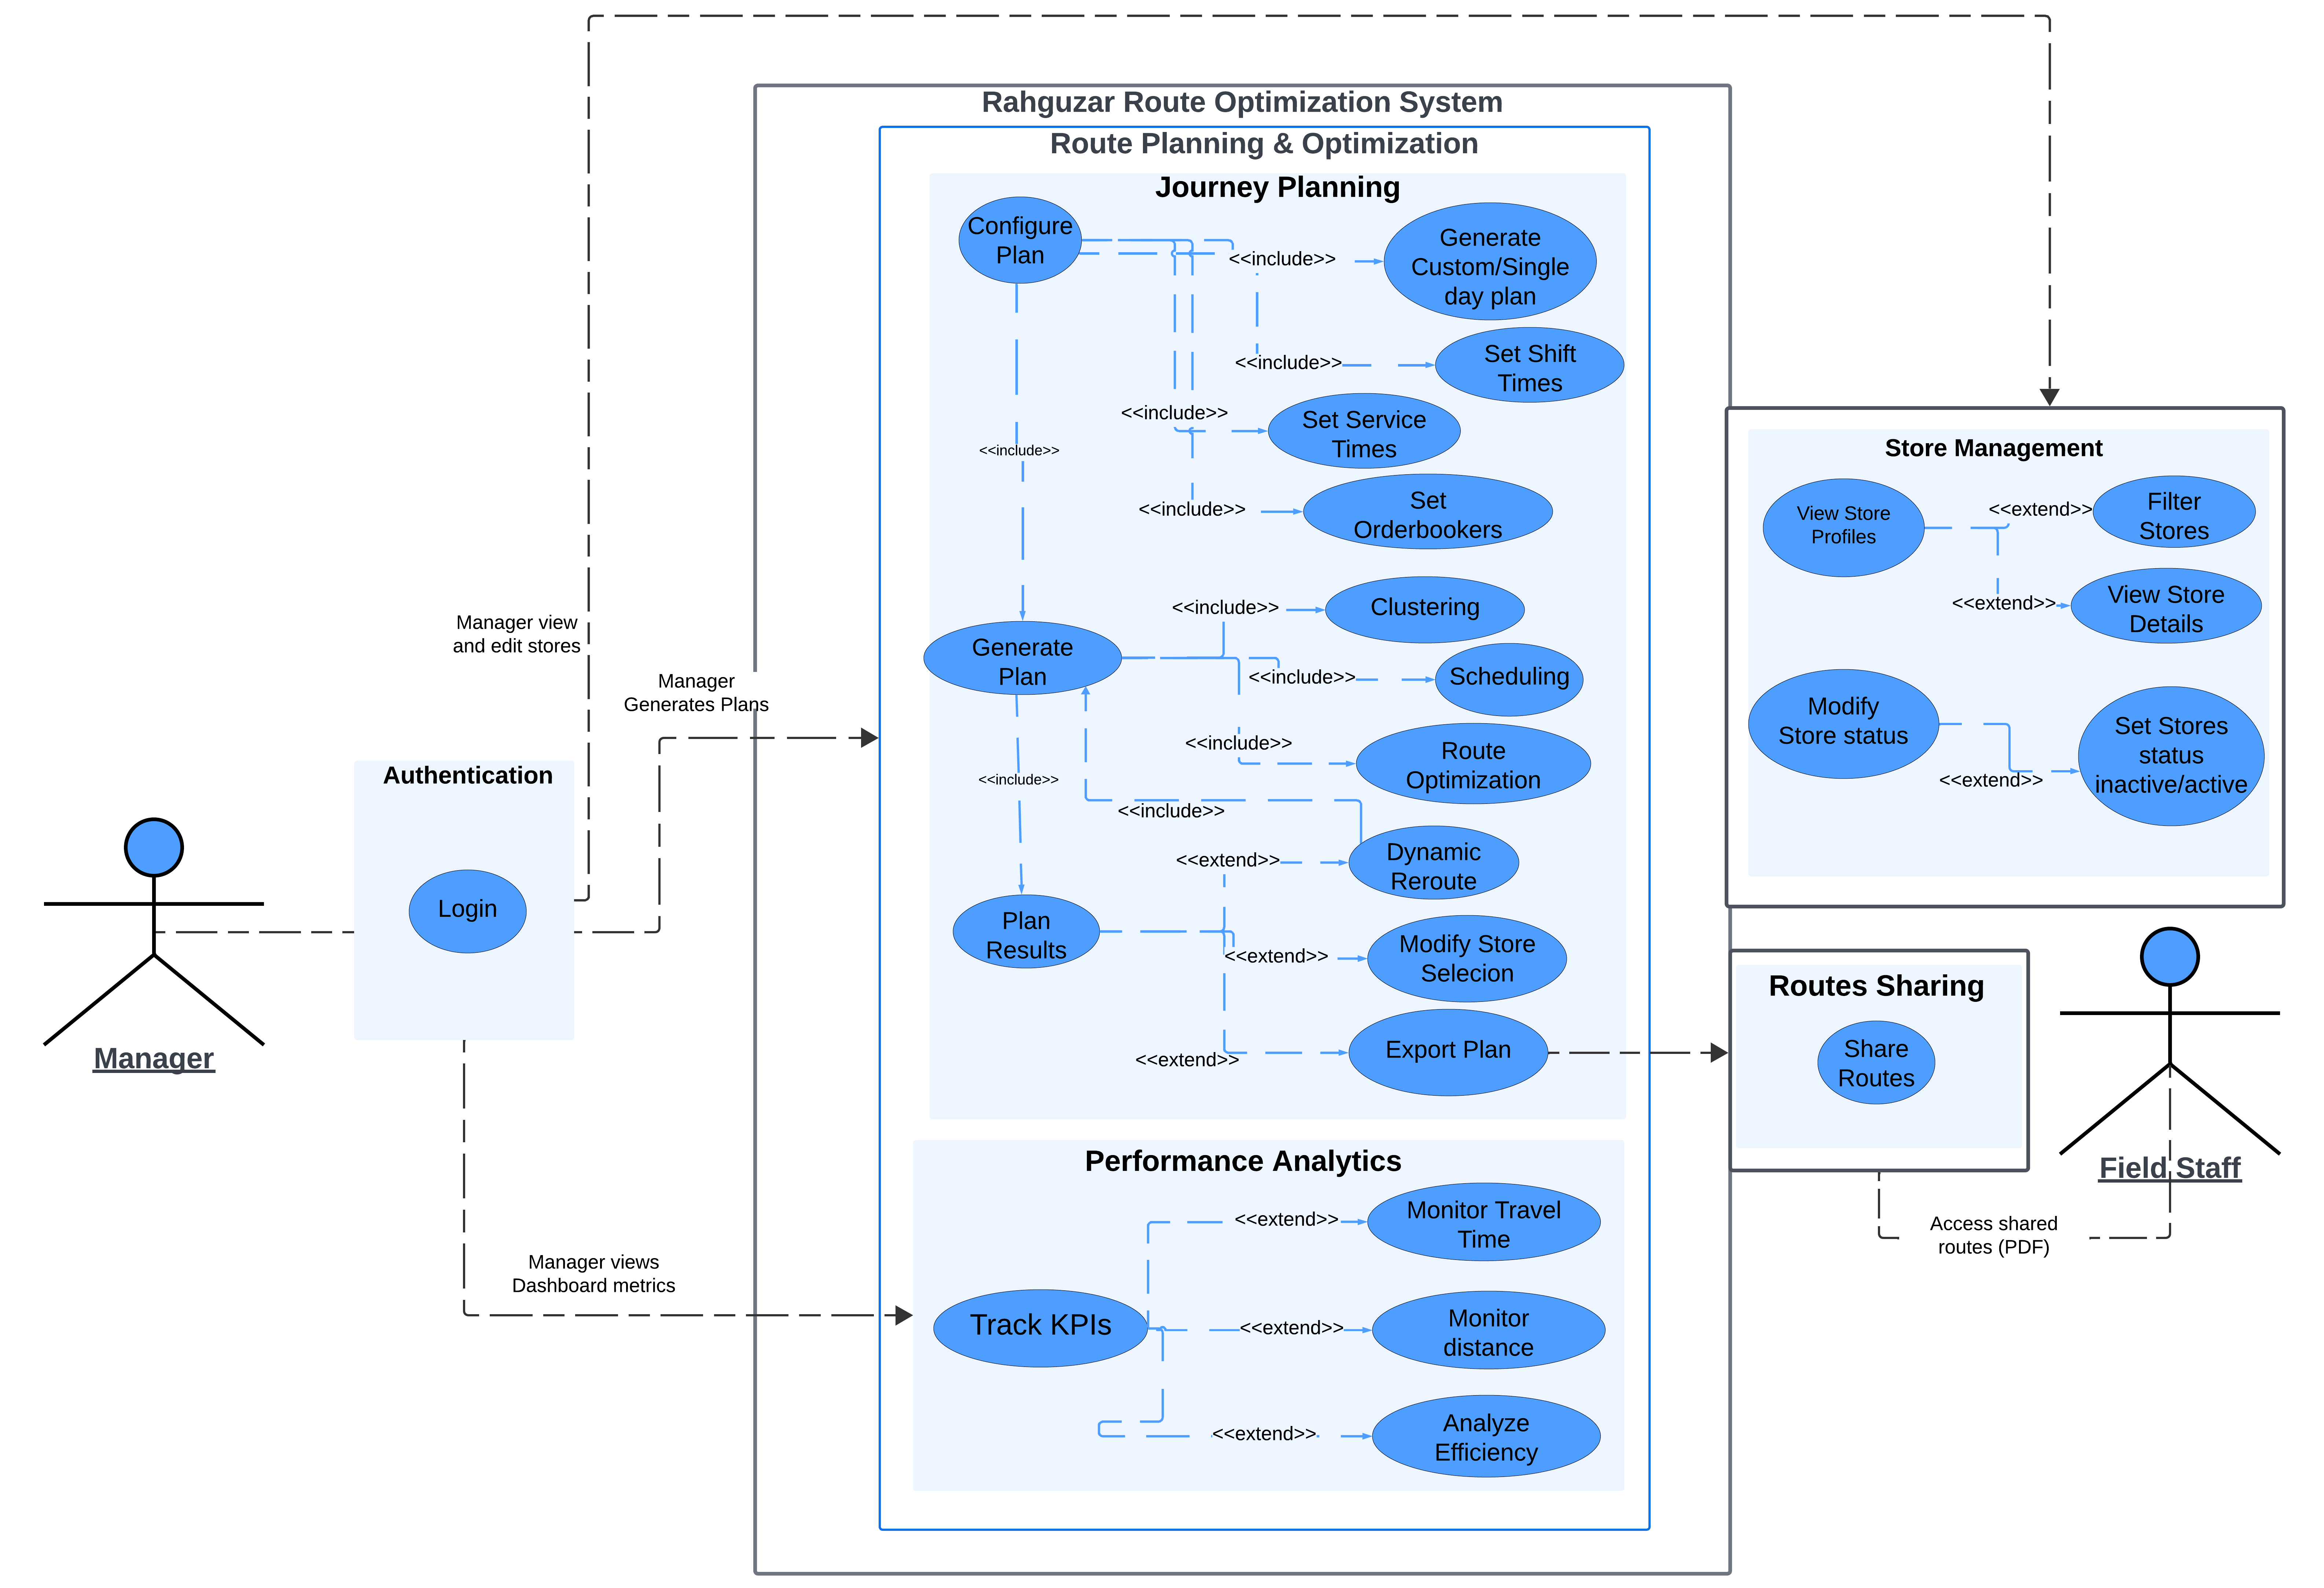
\includegraphics[width=0.98\textwidth]{images/Rahguzar - Use Case - Core System.png} 
        \caption{Rahguzar's Use Case Diagram}
    \end{figure}
\end{center}

\section{Datasets}
% This section describes the specific dataset(s) used to build our system. An appropriate snapshot of the dataset(s) is also included. Futher details, when needed, are presented in the appendix.
This section outlines the primary datasets that will support Rahguzar’s intelligent route planning and scheduling functionalities. These datasets provide crucial information on stores, visits, journey plans, and operational factors essential for optimized route generation. As per the NDA with SalesFlo, we are not permitted to share or disclose the data provided to us. 
\subsection*{Overview of Datasets}

\begin{enumerate}

\item \textbf{Store Universe} \\
This dataset provides foundational information on each store, including location, operational status, and distributor associations. Key fields include:
    \begin{itemize}
        \item \textbf{storecode:} Unique identifier for each store.
        \item \textbf{storestatus:} Operational status (active or inactive).
        \item \textbf{latitude and longitude:} Geographic coordinates.
        \item \textbf{distributorcode:} Code for the distributor linked to the store.
        \item \textbf{pjpcode:} Code for the Permanent Journey Plan (PJP) associated with the store.
    \end{itemize}
This dataset is essential for determining which stores to include in routes based on location and operational status.

\item \textbf{Store Hierarchy} \\
This dataset offers classification and hierarchical details, allowing route customization based on store attributes such as region or sales channel. Key fields include:
    \begin{itemize}
        \item \textbf{storecode:} Identifier for each store.
        \item \textbf{areatype, townid, localityid:} Geographical identifiers.
        \item \textbf{channeltypeid and channelid:} Sales channel identifiers (e.g., retail, wholesale).
        \item \textbf{storeclassificationIDs: } These classification IDs will be used to further distinguish between certain store categories.
    \end{itemize}
This data enables Rahguzar to organize routes by region and sales channel, optimizing for specific geographic and operational criteria.

\item \textbf{Visits} \\
The Visits dataset records historical visit information for each store, including time spent, visit order, and outcomes. Key fields include:
    \begin{itemize}
        \item \textbf{visitid:} Unique identifier for each visit.
        \item \textbf{pjpcode:} Journey plan code associated with the visit.
        \item \textbf{visitdate, visitstarttime, visitendtime:} Time data for analyzing visit durations.
        \item \textbf{visitspenttimeinseconds:} Total time spent at the store during the visit.
        \item \textbf{orderstatus:} Status of any order placed during the visit.
        \item \textbf{visiststatus: } Status determining if a visit has been completed or not.
        \item \textbf{syncdown, syncup, syncdowndatetime: } These fields track the synchronization status and timing of visit records: syncdown shows if data was downloaded to the device, syncup if it was uploaded to the server, and syncdowndatetime logs the last download timestamp.
    \end{itemize}
This dataset supports route optimization by providing insights into visit frequency and duration, refining future scheduling.

\end{enumerate}

% \subsection*{Additional Datasets Needed}

% To enhance Rahguzar's functionality, the following additional datasets may be required:

% \begin{enumerate}

% \item \textbf{Order Booker Shifts Dataset} \\
% This dataset contains information on the availability and shifts of order bookers. Key fields include:
%     \begin{itemize}
%         \item \textbf{bookerid:} Unique identifier for each order booker.
%         \item \textbf{shiftstarttime and shiftendtime:} Start and end times of each shift.
%         \item \textbf{availabilitystatus:} Indicates whether the booker is available or unavailable.
%     \end{itemize}
% This dataset is essential for scheduling routes within the working hours of each order booker, optimizing route generation according to workforce availability.

% \item \textbf{Geographic Data} \\
% Geographic and road network data provide detailed map and routing information, potentially sourced via the Google Maps API or GIS data services. Key components include:
%     \begin{itemize}
%         \item \textbf{roadnetwork:} Map of roads, including distances and travel times.
%         \item \textbf{trafficpatterns:} Historical traffic data for congestion analysis.
%         \item \textbf{geofencingdata:} Predefined boundaries for specific zones, regions, or territories.
%     \end{itemize}
% This dataset enables precise route calculations, factoring in real-time or historical traffic conditions to minimize travel time.

% \item \textbf{Store Activity Requirements} \\
% This dataset details the specific activities and time requirements for each store visit, allowing Rahguzar to optimize for different tasks performed at each store. Key fields include:
%     \begin{itemize}
%         \item \textbf{storecode:} Identifier for each store.
%         \item \textbf{activitytype:} Type of activity required (e.g., stock check, merchandising).
%         \item \textbf{estimatedtime:} Average time required to complete each activity.
%     \end{itemize}
% This dataset supports the system’s ability to tailor visit durations based on store requirements, leading to more accurate time estimates for each route.
% \end{enumerate}

\subsection*{Data Utilization in Rahguzar}

Together, these datasets will support Rahguzar’s core functionalities, including:
\begin{itemize}
    \item \textbf{Efficient Route Planning:} Leveraging store locations, operational statuses, and road networks for optimal routing.
    % \item \textbf{Dynamic Scheduling:} Using order booker shifts and activity requirements to generate flexible schedules aligned with store needs and workforce availability.
    \item \textbf{Traffic and Geographic Optimization:} Utilizing geographic data to plan routes that avoid congestion and optimize for specific zones or territories.
    % \item \textbf{Geographical Filtering:} Geographical and channel-based categorization from the Store Hierarchy dataset will help managers plan routes tailored to specific regions and sales priorities.
    \item \textbf{Route Efficiency Analysis:} The Visits dataset will provide insights into average visit durations and travel times, which will inform the route optimization algorithm and support KPI tracking for system performance.
\end{itemize}


\section{System Diagram}
\begin{center}
        \begin{figure}[H]
        \centering
        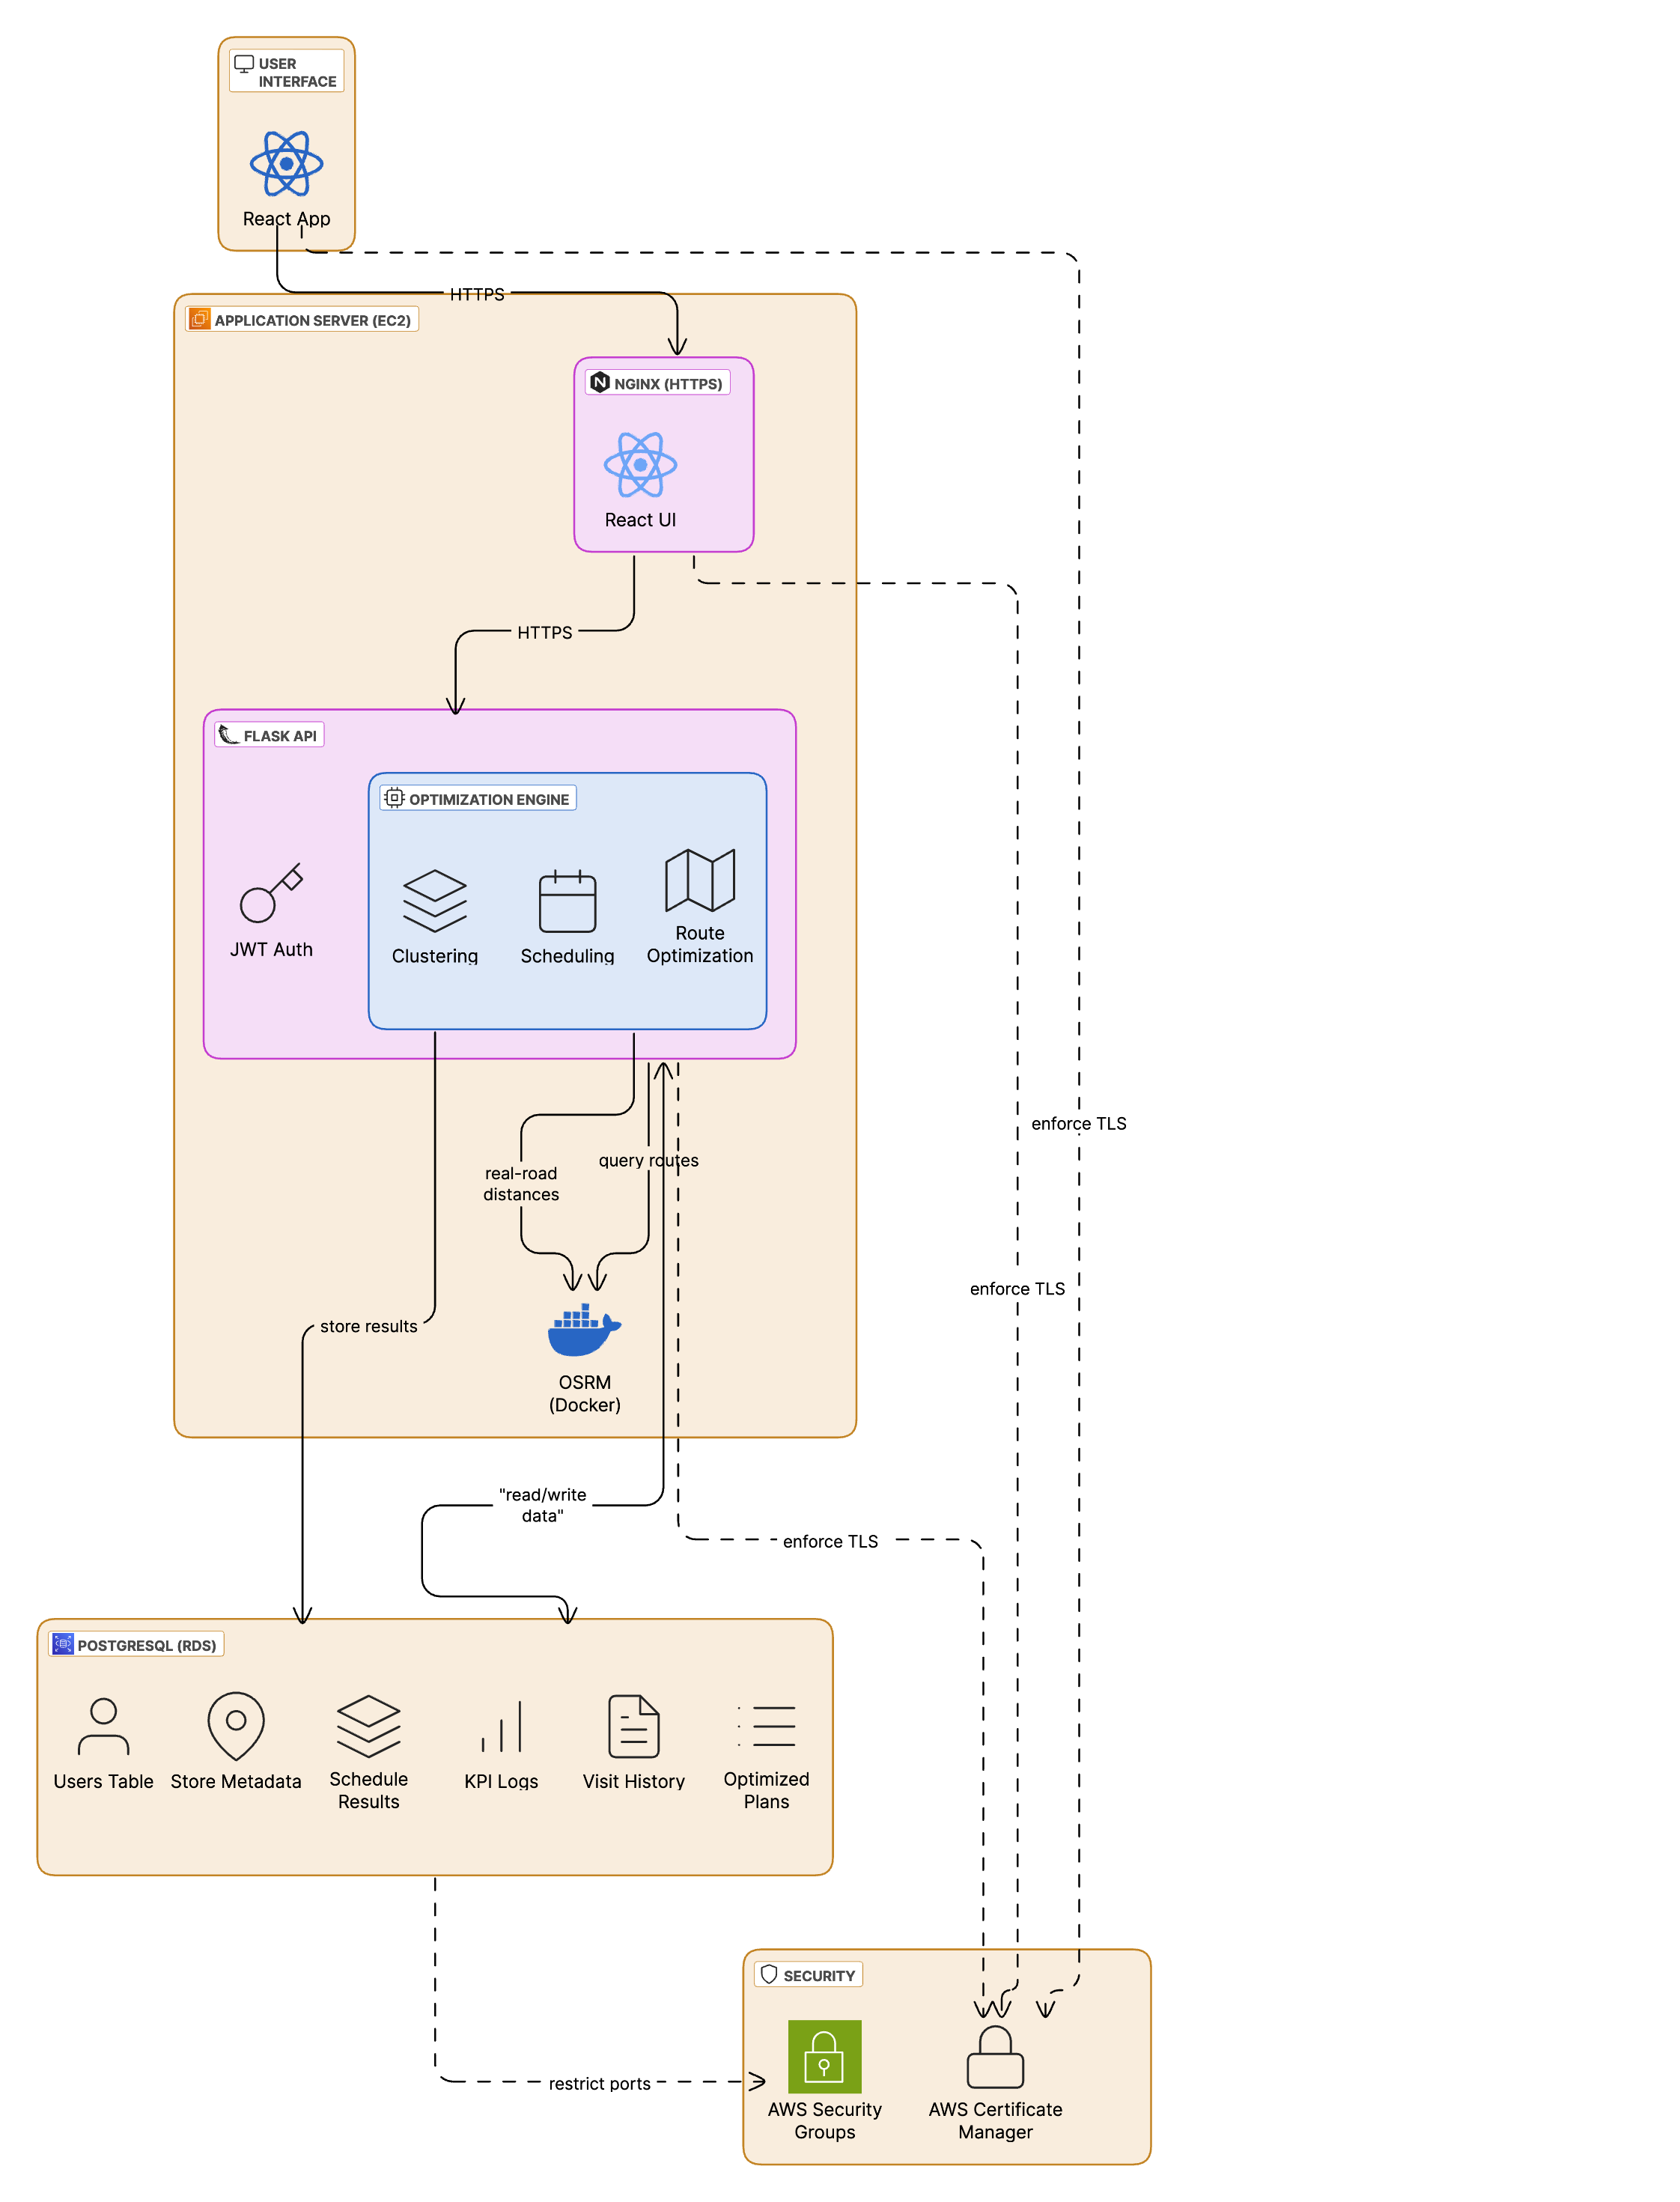
\includegraphics[width=\textwidth, height=0.75\textheight]{images/diagram.png} 
        \caption{Rahguzar's System Architecture Diagram}
    \end{figure}
\end{center}